% =============================================================================
%  Redação para o Exame de Qualificação de Mestrado
%  Gabriel Hernandez Rozo — FEQ/UNICAMP
%
%  Formatação reproduzindo o padrão da qualificação do Prof. Raphael Suppino
%  (2008), com citações e referências em ABNT (NBR 10520 / NBR 6023) via
%  abntex2cite.
%
%  Compilar: pdflatex -> bibtex -> pdflatex -> pdflatex
%  No Overleaf: selecionar pdfLaTeX e compilador de bibliografia BibTeX.
% =============================================================================

\documentclass[12pt,a4paper,oneside]{report}

% --- Codificação e idioma ----------------------------------------------------
\usepackage[T1]{fontenc}
\usepackage[utf8]{inputenc}
\usepackage[brazil]{babel}

% --- Tipografia --------------------------------------------------------------
\usepackage{mathptmx}                 % Times New Roman (texto e matemática)
\usepackage[scaled=0.90]{helvet}
\usepackage{courier}
\usepackage{microtype}

% --- Página ------------------------------------------------------------------
\usepackage[a4paper,top=2.5cm,bottom=2.5cm,left=3.0cm,right=2.5cm]{geometry}
\usepackage{setspace}
\onehalfspacing
\setlength{\parindent}{1.25cm}

% --- Matemática e tabelas ----------------------------------------------------
\usepackage{amsmath,amssymb}
\usepackage{booktabs}
\usepackage{multirow}
\usepackage{array}
\usepackage{siunitx}
\sisetup{output-decimal-marker={,}, per-mode=symbol, group-separator={\,}}

% --- Figuras -----------------------------------------------------------------
\usepackage{graphicx}
\usepackage{tikz}
\graphicspath{{figuras/}}
\usepackage{caption}
% Padrao Suppino (2008): legenda inteira em negrito, centralizada,
% separador em travessao. Figura com legenda abaixo; tabela, acima.
\captionsetup{font=bf, labelsep=endash, justification=centering,
               skip=10pt, singlelinecheck=false}

% --- Cabeçalhos --------------------------------------------------------------
\usepackage{fancyhdr}
\usepackage{emptypage}
\pagestyle{fancy}
\fancyhf{}
\fancyhead[L]{\itshape\nouppercase{\leftmark}}
\fancyhead[R]{\itshape\thepage}
\renewcommand{\headrulewidth}{0.8pt}
\fancypagestyle{plain}{%
  \fancyhf{}%
  \fancyhead[L]{\itshape\nouppercase{\leftmark}}%
  \fancyhead[R]{\itshape\thepage}%
  \renewcommand{\headrulewidth}{0.8pt}%
}

% --- Títulos de capítulo e seção ---------------------------------------------
\usepackage{titlesec}

\titleformat{\chapter}[display]
  {\normalfont\bfseries\centering}
  {\large Capítulo \thechapter}
  {0.4em}
  {\large}
\titlespacing*{\chapter}{0pt}{-20pt}{30pt}

\titleformat{name=\chapter,numberless}[display]
  {\normalfont\bfseries\centering}
  {}
  {0pt}
  {\large}
\titlespacing*{name=\chapter,numberless}{0pt}{-20pt}{30pt}

\titleformat{\section}
  {\normalfont\bfseries}
  {\thesection\ --}
  {0.4em}
  {}
\titlespacing*{\section}{0pt}{18pt}{10pt}

\titleformat{\subsection}
  {\normalfont\bfseries}
  {\thesubsection\ --}
  {0.4em}
  {}
\titlespacing*{\subsection}{0pt}{14pt}{8pt}

\renewcommand{\thesection}{\thechapter.\arabic{section}}

% --- Sumário e listas --------------------------------------------------------
\usepackage[titles]{tocloft}
\renewcommand{\cfttoctitlefont}{\hfill\bfseries\large}
\renewcommand{\cftaftertoctitle}{\hfill}
\renewcommand{\cftchapfont}{\bfseries}
\renewcommand{\cftchappagefont}{\bfseries}
\renewcommand{\cftchapdotsep}{\cftdotsep}
\setlength{\cftbeforechapskip}{8pt}

% --- Referências e citações (ABNT) -------------------------------------------
% biblatex-abnt implementa a NBR 6023:2018 e a NBR 10520:2002 e funciona com
% qualquer classe de documento. No Overleaf, o backend biber e detectado
% automaticamente a partir do \addbibresource.
\usepackage{csquotes}
\usepackage[backend=biber, style=abnt, giveninits=true]{biblatex}
\addbibresource{referencias.bib}

% --- Links -------------------------------------------------------------------
\usepackage[hidelinks,breaklinks]{hyperref}
\usepackage{url}

% --- Marcador de pendência ---------------------------------------------------
% Trechos que ainda dependem de dado experimental ou de referência a confirmar.
% Para a versão final, trocar a definição por \newcommand{\pendente}[1]{}
\usepackage[table]{xcolor}
\newcommand{\pendente}[1]{\textcolor{red}{\textbf{[PENDENTE:} #1\textbf{]}}}

% --- Ajustes finais ----------------------------------------------------------
\renewcommand{\chaptermark}[1]{\markboth{Capítulo \thechapter\ -- #1}{}}
\renewcommand{\bibname}{Referências Bibliográficas}

\begin{document}

% =============================== PRÉ-TEXTUAL =================================
\pagenumbering{roman}
\pagestyle{empty}
\begin{titlepage}
\begin{center}

{\large\bfseries UNIVERSIDADE ESTADUAL DE CAMPINAS}\\[2pt]
{\large\bfseries FACULDADE DE ENGENHARIA QUÍMICA}\\[14pt]

{\normalsize ÁREA DE CONCENTRAÇÃO: \pendente{confirmar a área de concentração do programa}}

\vspace{4.5cm}

{\normalsize
MODELAGEM FLUIDODINÂMICA COMPUTACIONAL DE UM REATOR\\
MONOLÍTICO DE PAREDE CATALÍTICA PARA A PRODUÇÃO DE\\
BIODIESEL POR TRANSESTERIFICAÇÃO HETEROGÊNEA
}

\vspace{4.5cm}

\end{center}

\noindent\textbf{Autor:} Gabriel Hernandez Rozo\\[4pt]
\noindent\textbf{Orientador:} Prof. Dr. Raphael Soeiro Suppino\\[4pt]
\noindent\textbf{Coorientador:} Prof. Dr. Dirceu Noriler

\vspace{2.0cm}

\noindent\parbox{\textwidth}{\normalsize
Redação para o Exame de Qualificação de Mestrado apresentada à Comissão de
Pós-Graduação da Faculdade de Engenharia Química como parte dos requisitos
para obtenção do título de Mestre em Engenharia Química.}

\vfill

\begin{center}
Campinas -- São Paulo\\
Dezembro de 2026
\end{center}

\end{titlepage}


\pagestyle{fancy}
\cleardoublepage
\markboth{Sumário}{}
\tableofcontents

\cleardoublepage
\markboth{Lista de Figuras}{}
\addcontentsline{toc}{chapter}{Lista de Figuras}
\listoffigures

\cleardoublepage
\markboth{Lista de Tabelas}{}
\addcontentsline{toc}{chapter}{Lista de Tabelas}
\listoftables

\cleardoublepage
\chapter*{Nomenclatura}
\addcontentsline{toc}{chapter}{Nomenclatura}
\markboth{Nomenclatura}{}

\vspace{-10pt}
\noindent\textbf{Letras latinas}
\begin{center}
\renewcommand{\arraystretch}{1.35}
\begin{tabular}{p{2.2cm} p{8.6cm} p{3.0cm}}
\hline
Símbolo & Significado & Unidade \\
\hline
$A_p$        & Área da parede catalítica                              & \si{\meter\squared} \\
$C_i$        & Concentração molar da espécie $i$                      & \si{\kilo\mole\per\meter\cubed} \\
$D_h$        & Diâmetro hidráulico do canal                           & \si{\meter} \\
$D_i$        & Difusividade mássica efetiva da espécie $i$            & \si{\meter\squared\per\second} \\
$D_p$        & Difusividade efetiva no interior do \textit{washcoat}  & \si{\meter\squared\per\second} \\
$Da$         & Número de Damköhler de parede                          & -- \\
$H$          & Altura do canal                                        & \si{\meter} \\
$J_i$        & Fluxo mássico da espécie $i$ na parede                 & \si{\kilogram\per\meter\squared\per\second} \\
$k_{cat}$    & Constante cinética por massa de catalisador            & \si{\meter\cubed\per\kilogram\per\second} \\
$k_m$        & Coeficiente de transferência de massa                  & \si{\meter\per\second} \\
$k_v$        & Constante cinética por volume de \textit{washcoat}     & \si{\per\second} \\
$L$          & Comprimento do canal                                   & \si{\meter} \\
$L_e$        & Comprimento de entrada mássica                         & \si{\meter} \\
$M_i$        & Massa molar da espécie $i$                             & \si{\kilogram\per\kilo\mole} \\
$\dot{m}$    & Vazão mássica                                          & \si{\kilogram\per\second} \\
$p$          & Pressão                                                & \si{\pascal} \\
$Pe$         & Número de Péclet mássico                               & -- \\
$Re$         & Número de Reynolds                                     & -- \\
$r_w$        & Taxa de reação por área de parede                      & \si{\kilo\mole\per\meter\squared\per\second} \\
$Sc$         & Número de Schmidt                                      & -- \\
$T$          & Temperatura                                            & \si{\kelvin} \\
$t$          & Tempo                                                  & \si{\second} \\
$\mathbf{u}$ & Vetor velocidade                                       & \si{\meter\per\second} \\
$\bar{u}$    & Velocidade média na seção                              & \si{\meter\per\second} \\
$w$          & Massa de catalisador por área de parede                & \si{\kilogram\per\meter\squared} \\
$X_{TG}$     & Conversão de triglicerídeo                             & -- \\
$x$          & Coordenada axial                                       & \si{\meter} \\
$Y_i$        & Fração mássica da espécie $i$                          & -- \\
$y$          & Coordenada transversal                                 & \si{\meter} \\
\hline
\end{tabular}
\end{center}

\vspace{6pt}
\noindent\textbf{Letras gregas}
\begin{center}
\renewcommand{\arraystretch}{1.35}
\begin{tabular}{p{2.2cm} p{8.6cm} p{3.0cm}}
\hline
Símbolo & Significado & Unidade \\
\hline
$\gamma$        & Taxa de cisalhamento junto à parede        & \si{\per\second} \\
$\delta_c$      & Espessura da camada-limite de concentração & \si{\meter} \\
$\delta_{wc}$   & Espessura do \textit{washcoat}             & \si{\meter} \\
$\eta$          & Fator de efetividade do \textit{washcoat}  & -- \\
$\mu$           & Viscosidade dinâmica                       & \si{\pascal\second} \\
$\nu$           & Viscosidade cinemática                     & \si{\meter\squared\per\second} \\
$\rho$          & Massa específica do meio reacional         & \si{\kilogram\per\meter\cubed} \\
$\rho_{wc}$     & Massa específica do \textit{washcoat}      & \si{\kilogram\per\meter\cubed} \\
$\phi$          & Módulo de Thiele                           & -- \\
\hline
\end{tabular}
\end{center}

\vspace{6pt}
\noindent\textbf{Siglas e abreviaturas}
\begin{center}
\renewcommand{\arraystretch}{1.35}
\begin{tabular}{p{2.2cm} p{11.6cm}}
\hline
Sigla & Significado \\
\hline
CFD   & Fluidodinâmica computacional (\textit{Computational Fluid Dynamics}) \\
cpsi  & Células por polegada quadrada (\textit{cells per square inch}) \\
FAME  & Éster metílico de ácido graxo (\textit{Fatty Acid Methyl Ester}) \\
GL    & Glicerol \\
MeOH  & Metanol \\
TG    & Triglicerídeo \\
\hline
\end{tabular}
\end{center}


\cleardoublepage
\chapter*{Resumo}
\addcontentsline{toc}{chapter}{Resumo}
\markboth{Resumo}{}

A produção de biodiesel por transesterificação alcalina homogênea, rota
predominante na indústria, esbarra em dificuldades conhecidas de separação e
purificação, além de gerar efluentes que precisam ser neutralizados. A
substituição do catalisador dissolvido por um sólido elimina boa parte desses
inconvenientes, mas introduz em seu lugar um problema de transporte: os
reagentes passam a depender da difusão até a superfície ativa, e o óleo vegetal,
cuja difusividade mássica é cinco ordens de grandeza menor que a difusividade de
momento, não é um meio favorável a esse tipo de transporte.

Reatores monolíticos de parede catalítica oferecem uma resposta possível a esse
problema, por combinarem elevada razão entre área superficial e volume com perda
de carga reduzida. A pergunta que o presente trabalho procura responder é se a
geometria monolítica de fato se justifica para a transesterificação do óleo de
soja com óxido de cálcio, ou se o sistema opera em um regime no qual a área
adicional não é aproveitada.

O trabalho é conduzido por meio de simulação fluidodinâmica computacional de um
canal representativo do monólito, em regime laminar e isotérmico a \SI{65}{\celsius},
com o catalisador tratado como condição de contorno de fluxo de espécies na
parede. A resistência difusional no interior do \textit{washcoat} é incorporada
por um fator de efetividade calculado a partir do módulo de Thiele, o que evita
discretizar a camada porosa. Os parâmetros cinéticos provêm de medidas
realizadas no próprio laboratório com CaO suportado em biochar.

Os resultados preliminares indicam que o número de Damköhler de parede vale
\num{0.76}, o que situa o sistema em regime misto: a resistência cinética e a
resistência ao transporte externo são da mesma ordem, e a concentração de
triglicerídeo junto à superfície catalítica é \SI{43}{\percent} menor que no seio
do fluido. Esse valor foi reproduzido em duas malhas independentes e em duas
composições de alimentação distintas, com discrepância inferior a
\SI{2}{\percent}. Verificou-se ainda que o comprimento de entrada mássica do
canal simulado é de \SI{3.46}{\meter}, contra os \SI{50}{\milli\meter} de
comprimento físico, de modo que a camada-limite de concentração jamais se
desenvolve e a conversão por passe permanece baixa, em torno de
\SI{1.4}{\percent}.

Nas etapas seguintes, o modelo será calibrado contra os dados experimentais em
obtenção no laboratório, estendido à varredura de temperatura e de espessura de
\textit{washcoat}, e empregado para a avaliação de geometrias alternativas de
canal.

\vspace{10pt}
\noindent\textbf{Palavras-chave:} biodiesel; transesterificação heterogênea;
reator monolítico; fluidodinâmica computacional; número de Damköhler.


% ================================ TEXTUAL ====================================
\cleardoublepage
\pagenumbering{arabic}
\setcounter{page}{1}

\chapter*{Introdução}
\addcontentsline{toc}{chapter}{Introdução}
\markboth{Introdução}{}

O biodiesel é obtido industrialmente pela transesterificação de óleos vegetais
ou gorduras animais com um álcool de cadeia curta, quase sempre o metanol, na
presença de um catalisador básico dissolvido no meio reacional. A rota é madura
e opera com rendimentos elevados em tempos de reação curtos, mas carrega
dificuldades que são bem conhecidas de quem a pratica. O catalisador homogêneo
não pode ser recuperado ao fim da reação e precisa ser neutralizado, o que
consome ácido e gera sais. A separação da glicerina exige lavagens sucessivas, e
a água empregada nessas lavagens retorna ao processo como efluente. Quando a
matéria-prima contém ácidos graxos livres em teor apreciável, parte do
catalisador é consumida na formação de sabões, que estabilizam emulsões e
dificultam ainda mais a separação das fases.

A substituição do catalisador dissolvido por um sólido resolve a maior parte
desses problemas de uma só vez. O catalisador deixa de contaminar os produtos,
pode ser retido no reator e reutilizado, e a etapa de neutralização desaparece.
Entre os sólidos básicos estudados para essa finalidade, o óxido de cálcio tem
recebido atenção particular por reunir basicidade adequada, baixo custo e
disponibilidade a partir de fontes residuais, como cascas de ovo e conchas
calcinadas. O preço dessa substituição, entretanto, é a introdução de uma
resistência que a rota homogênea não possui: os reagentes precisam alcançar a
superfície ativa por difusão, e só então reagir.

Essa resistência não é desprezível no caso em questão. Óleos vegetais são
líquidos viscosos cujas moléculas de triglicerídeo têm massa molar próxima de
\SI{870}{\gram\per\mole}, e a difusividade mássica correspondente é da ordem de
\SI{1e-11}{\meter\squared\per\second}. Comparada à difusividade de momento do
mesmo meio, essa grandeza é cerca de cem mil vezes menor, o que coloca o sistema
em uma faixa de número de Schmidt incomum na prática de engenharia de reatores.
Em termos operacionais, isso significa que o transporte de reagente até a parede
catalítica pode se tornar a etapa mais lenta do conjunto, independentemente de
quão ativo seja o catalisador empregado.

É nesse ponto que a configuração do reator deixa de ser um detalhe de projeto.
Reatores monolíticos de parede catalítica, formados por um feixe de canais
paralelos de pequeno diâmetro cujas paredes são recobertas por uma camada fina
de catalisador, oferecem razão entre área superficial e volume muito superior à
de um leito fixo convencional, com perda de carga substancialmente menor. A
área adicional, contudo, só se traduz em desempenho quando existe de fato um
gradiente de concentração a ser vencido. Se o sistema estiver sob controle
cinético estrito, a reação é lenta o bastante para que o reagente alcance a
parede sem dificuldade, e a geometria do monólito não cumpre função alguma que
justifique sua complexidade de fabricação.

Decidir em qual desses regimes o sistema opera não é algo que se resolva por
inspeção. A resposta depende simultaneamente da atividade do catalisador, da
espessura e da porosidade da camada depositada, da geometria do canal e da
velocidade de escoamento, e as grandezas envolvidas percorrem várias ordens de
grandeza. A fluidodinâmica computacional permite tratar esse acoplamento de
forma explícita, resolvendo o campo de concentração no interior do canal com a
reação heterogênea imposta como condição de contorno na parede, e extraindo daí
os grupos adimensionais que caracterizam o regime.

No grupo de pesquisa em que este trabalho se insere, a transesterificação
heterogênea com óxido de cálcio vem sendo investigada experimentalmente há
alguns anos. \citeonline{Melo2023} determinou parâmetros cinéticos para a
metanólise de óleo de soja sobre CaO suportado em biochar a \SI{65}{\celsius},
e \citeonline{Fonseca2026} estendeu o estudo à rota etílica com CaO e
CaO/Al$_2$O$_3$, reportando difusividades efetivas no interior de catalisadores
dessa natureza. Esses dois conjuntos de dados fornecem os parâmetros necessários
para alimentar um modelo de reator, e é sobre eles que o presente trabalho se
apoia.

O objetivo geral desta dissertação é avaliar, por meio de simulação
fluidodinâmica computacional, o desempenho de um reator monolítico de parede
catalítica aplicado à transesterificação heterogênea de óleo de soja com óxido
de cálcio, identificando o regime de operação do sistema e as variáveis de
projeto que o governam. São objetivos específicos:

\begin{itemize}
\itemsep2pt
\item construir um modelo de canal representativo do monólito que resolva
      simultaneamente o escoamento e o transporte multicomponente de espécies,
      com a reação heterogênea tratada como condição de contorno de parede;
\item incorporar a resistência difusional interna ao \textit{washcoat} por meio
      de um fator de efetividade, evitando a discretização da camada porosa;
\item verificar o modelo quanto à conservação de massa, à independência de
      malha e ao fechamento do balanço global por espécie;
\item determinar o número de Damköhler de parede e classificar o regime de
      operação do sistema com os parâmetros cinéticos do catalisador
      efetivamente empregado no laboratório;
\item avaliar a influência da espessura do \textit{washcoat}, da temperatura e
      da geometria do canal sobre a conversão por passe;
\item calibrar o modelo contra os dados experimentais obtidos no laboratório.
\end{itemize}

Nesta redação para o Exame de Qualificação, o Capítulo~\ref{cap:revisao}
apresenta uma revisão da literatura sobre a transesterificação heterogênea, os
catalisadores sólidos básicos empregados na reação e a modelagem de reatores de
parede catalítica, com atenção particular aos grupos adimensionais que
caracterizam a competição entre reação e transporte. O Capítulo~\ref{cap:modelagem}
descreve o modelo matemático construído, as hipóteses adotadas, a implementação
numérica e os testes de verificação aplicados. No Capítulo~\ref{cap:resultados}
reúnem-se os resultados preliminares já obtidos, que incluem a validação
hidrodinâmica do modelo, a determinação do regime de operação e a caracterização
da camada-limite de concentração. O Capítulo~\ref{cap:cronograma} apresenta os
resultados esperados para as etapas restantes e o cronograma previsto para sua
execução.

\chapter{Revisão Bibliográfica}
\label{cap:revisao}

\section{A reação de transesterificação}

A transesterificação de um triglicerídeo com um álcool de cadeia curta produz
ésteres alquílicos de ácidos graxos e glicerol. Empregando-se metanol, a reação
global é escrita como

\begin{equation}
\mathrm{TG} + 3\,\mathrm{MeOH} \rightleftharpoons 3\,\mathrm{FAME} + \mathrm{GL}
\label{eq:global}
\end{equation}

\noindent
em que TG designa o triglicerídeo, FAME o éster metílico e GL o glicerol. A
estequiometria global, contudo, esconde o que de fato ocorre no meio reacional.
A conversão se dá por três etapas consecutivas e reversíveis, nas quais o
triglicerídeo é sucessivamente convertido a diglicerídeo, monoglicerídeo e
glicerol, liberando uma molécula de éster a cada passagem
\parencite{Noureddini1997}:

\begin{align}
\mathrm{TG}  + \mathrm{MeOH} &\rightleftharpoons \mathrm{DG} + \mathrm{FAME} \label{eq:etapa1}\\
\mathrm{DG}  + \mathrm{MeOH} &\rightleftharpoons \mathrm{MG} + \mathrm{FAME} \label{eq:etapa2}\\
\mathrm{MG}  + \mathrm{MeOH} &\rightleftharpoons \mathrm{GL} + \mathrm{FAME} \label{eq:etapa3}
\end{align}

O caráter reversível das três etapas impõe o emprego de excesso de álcool para
deslocar o equilíbrio na direção dos produtos. Razões molares entre
\num{6}:\num{1} e \num{12}:\num{1} de álcool para óleo são as mais comuns na
prática, contra o valor estequiométrico de \num{3}:\num{1}
\parencite{Freedman1986}. O excesso cumpre ainda uma segunda função, menos evidente:
ao manter a concentração de metanol praticamente constante ao longo da reação,
permite que a cinética seja tratada como de pseudo-primeira ordem no
triglicerídeo, simplificação de que este trabalho faz uso no
Capítulo~\ref{cap:modelagem}.

O excesso não é, entretanto, gratuito. Como observam \textcite{Allain2016}, o
álcool não convertido precisa ser recuperado a jusante do reator, e essa
separação responde por parcela apreciável do consumo energético do processo.
Em catálise heterogênea o excesso tende a ser ainda maior, justamente porque a
reação passa a ser limitada também pela difusão até o catalisador. Há portanto
um compromisso entre conversão por passe e custo de separação, que o projeto do
reator pode deslocar.

A escolha do modelo cinético empregado para descrever essa sequência não é
arbitrária, e \textcite{Ezzati2021} a sistematizaram em bases teóricas. Partindo
do mecanismo de três etapas, os autores derivaram uma equação de taxa geral,
válida ao longo de todo o tempo de reação, e mostraram a quais condições cada
modelo simplificado corresponde: a equação geral reduz-se ao modelo de segunda
ordem nos tempos iniciais de reação, e ao modelo de pseudo-primeira ordem nos
tempos iniciais com álcool em alta concentração. A conclusão que interessa
diretamente a este trabalho é a restrição: ao contrário do que a prática
corrente sugere, os modelos de pseudo-primeira e de segunda ordem são acurados
apenas nos tempos iniciais de reação, e não ao longo de toda ela.

Essa restrição é satisfeita no sistema aqui estudado, e por uma razão que
decorre do próprio resultado obtido. Como se mostra no
Capítulo~\ref{cap:resultados}, a conversão por passe no canal monolítico é de
\SI{1.4}{\percent}, de modo que o fluido percorre o reator permanecendo no
regime de tempos iniciais a que a aproximação de pseudo-primeira ordem se
aplica. A hipótese adotada na Seção~\ref{sec:bc} apoia-se nessa coincidência, e
deixaria de valer caso configurações de conversão elevada viessem a ser
simuladas.

Entre os fatores que governam o rendimento da reação, \textcite{Freedman1986}
identificaram a razão molar álcool/óleo, a temperatura, o teor de catalisador e
a presença de água e de ácidos graxos livres na matéria-prima. A temperatura de
operação é limitada superiormente pelo ponto de ebulição do metanol, de
\SI{64.7}{\celsius} à pressão atmosférica, de modo que a maior parte dos
trabalhos opera próximo a \SI{60}{\celsius} em sistema aberto, ou em pressões
moderadas quando se deseja ultrapassar esse limite.

\section{Limitações da rota homogênea}

A catálise alcalina homogênea, conduzida com hidróxido ou metóxido de sódio ou
potássio dissolvidos no metanol, continua a ser a rota predominante na indústria
por razões de desempenho. As velocidades de reação são elevadas, e conversões
superiores a \SI{95}{\percent} são alcançadas em menos de uma hora a
\SI{60}{\celsius}.

As dificuldades aparecem a jusante do reator. O catalisador permanece dissolvido
nos produtos e precisa ser neutralizado com ácido, operação que consome insumo e
gera uma corrente salina. A glicerina obtida carrega sais e metanol residual, o
que reduz seu valor comercial e exige purificação adicional. A separação das
fases demanda lavagens sucessivas com água, cuja corrente de saída retorna ao
processo como efluente a ser tratado.

Matérias-primas de menor custo agravam o quadro. Óleos residuais e gorduras
animais contêm ácidos graxos livres em teores que podem superar
\SI{5}{\percent}, e esses ácidos consomem o catalisador básico na formação de
sabões. Além de reduzir a quantidade de catalisador disponível para a reação
pretendida, os sabões formados estabilizam emulsões entre as fases éster e
glicerol, dificultando a separação e reduzindo o rendimento efetivo do processo.

\pendente{acrescentar dados quantitativos de consumo de insumos e geração de
efluentes, que as referências consultadas até aqui não trazem de forma
consolidada}

\subsection{A mistura bifásica e a limitação por transferência interfacial}
\label{sec:bifasico}

Há uma dificuldade anterior a todas as mencionadas, e que independe da natureza
do catalisador. Óleo vegetal e metanol têm polaridades muito distintas e
apresentam lacuna de miscibilidade: a mistura inicial de reagentes não é uma
solução, e sim um sistema líquido-líquido de duas fases, uma rica em óleo e
outra rica em álcool \cite{Muller2019}.

A consequência é que a taxa global passa a depender da transferência de massa
através da interface entre as fases, que é lenta em comparação com a reação
química. \textcite{Muller2019} observa que a etapa inicial da reação é
caracterizada por limitações difusionais severas, decorrentes justamente dessa
solubilidade mútua reduzida, e que o aumento da área interfacial por meios
mecânicos --- agitação, misturadores estáticos, sonicação, microrreatores ---
constitui a resposta habitual ao problema.

A situação se altera ao longo da conversão. Os ésteres formados atuam como
cossolvente entre as duas fases, e \textcite{Muller2019} registra que a mistura
se torna homogênea quando a reação atinge algo entre
\SIrange{15}{20}{\percent} de conversão, a partir do que a necessidade de mistura
intensiva diminui. A conversões ainda mais altas, o éster se separa da
glicerina, e o sistema volta a ser bifásico por outra razão.

Essa transição tem implicação direta sobre o presente trabalho, e é retomada na
Seção~\ref{sec:limitacoes}.

Registre-se, por fim, que a configuração de reator responde a essas
dificuldades de formas distintas. \textcite{Muller2019} contrasta a operação em
batelada, flexível quanto à matéria-prima mas de baixa produtividade e com
variação de qualidade entre bateladas, com a operação contínua, que oferece
qualidade mais constante e menor custo operacional por unidade de produto ao
preço de maior investimento e de controle de processo mais elaborado. Entre os
reatores contínuos, aponta os de leito fixo tubular como introduzidos
precisamente para superar as limitações intrínsecas de conversão dos reatores
com retromistura.

\section{Catálise heterogênea com óxido de cálcio}
\label{sec:cao}

A imobilização do catalisador em uma fase sólida elimina, de uma só vez, a
neutralização, a contaminação da glicerina e boa parte das lavagens. O
catalisador pode ser recuperado por filtração ou, no caso de um reator de leito
fixo ou de parede catalítica, simplesmente permanece no equipamento.

Entre os sólidos básicos investigados para a reação, o óxido de cálcio reúne
características que explicam sua posição de destaque na literatura: basicidade
suficiente para catalisar a reação em temperaturas brandas, custo baixo,
toxicidade reduzida e possibilidade de obtenção a partir de resíduos
carbonáticos, como cascas de ovo, conchas e carapaças, por calcinação. A
atividade do CaO está associada aos sítios básicos de Lewis formados pelos
pares O$^{2-}$ na superfície, que abstraem o próton do metanol e geram o íon
metóxido, espécie que efetivamente ataca o carbono carbonílico do
triglicerídeo.

Duas limitações do CaO são recorrentemente apontadas. A primeira é a lixiviação
de cálcio para o meio reacional, que introduz uma contribuição homogênea à
conversão observada e reduz a vida útil do catalisador ao longo de ciclos
sucessivos. A segunda é a sensibilidade à água e ao dióxido de carbono
atmosféricos, que convertem a superfície a hidróxido e a carbonato,
desativando-a; por essa razão o catalisador é normalmente calcinado
imediatamente antes do uso.

A lixiviação foi quantificada por \textcite{Melo2023} em condições próximas das
aqui simuladas. Medindo o teor de Ca$^{2+}$ no biodiesel produzido, o autor
obteve \SI{585(375)}{\milli\gram\per\kilogram} para o CaO não suportado e
\SI{40(26)}{\milli\gram\per\kilogram} para o CaO depositado em biochar de bagaço
de cana. Os dois valores excedem o limite de \num{5} ppm fixado pela
ANP n\textsuperscript{o} 45/2014, pela ASTM D6751 e pela EN 14214, mas o suporte
reduz o arraste de cálcio por um fator próximo de quinze. O autor atribui essa
retenção aos grupos funcionais oxigenados do biochar ativado, que ancorariam o
cálcio à matriz carbonácea, possivelmente por ligações O--Ca--O.

A desativação ao longo de ciclos sucessivos tem origem distinta da lixiviação, e
igualmente relevante para a operação contínua. \textcite{Melo2023} observou
queda acentuada de atividade entre ciclos, chegando a \SI{49.4}{\percent} de
conversão no segundo e a conversão nula no terceiro, a depender do procedimento
de lavagem empregado, e atribuiu o efeito ao acúmulo de glicerídeos e glicerol
aderidos à superfície do catalisador, confirmado por microscopia eletrônica.
Nenhum dos cinco procedimentos de lavagem ensaiados restabeleceu plenamente a
atividade.

Esses dois mecanismos, arraste de cálcio e bloqueio da superfície, não são
tratados pelo modelo desenvolvido neste trabalho, que é isotérmico e de estado
quase-estacionário. Condicionam, porém, a viabilidade prática da configuração e
definem o horizonte de operação que o reator pode sustentar antes de exigir
regeneração.

Duas dissertações recentes do mesmo programa de pós-graduação forneceram os
parâmetros empregados na presente modelagem.
\textcite{Melo2023} estudou a metanólise de óleo de soja sobre CaO suportado
em biochar a \SI{65}{\celsius}, obtendo a constante cinética por massa de
catalisador adotada no Capítulo~\ref{cap:modelagem}. \textcite{Fonseca2026}
investigou a rota etílica com CaO e CaO/Al$_2$O$_3$ a \SI{70}{\celsius} e razão
molar óleo:etanol de \num{1}:\num{9}, reportando difusividades efetivas no
interior do catalisador na faixa de \SIrange{3e-13}{4.4e-12}{\meter\squared\per\second},
valores que sustentam a estimativa do fator de efetividade apresentada na
Seção~\ref{sec:thiele}.

\section{Reatores monolíticos de parede catalítica}

Um monólito catalítico consiste em um bloco cerâmico ou metálico atravessado por
um grande número de canais paralelos de seção reta pequena, cujas paredes são
recobertas por uma camada fina de material catalítico, denominada
\textit{washcoat}. A densidade de canais é expressa em células por polegada
quadrada, e valores entre \num{200} e \num{600}~cpsi são usuais.

A geometria oferece duas vantagens sobre o leito fixo convencional. A razão
entre área superficial e volume é consideravelmente maior, o que aumenta a área
disponível para reação por unidade de volume de reator. E, como o escoamento se
dá em canais retos e abertos, a perda de carga é muito inferior à de um leito de
partículas, o que reduz o custo de bombeamento e viabiliza vazões elevadas.

A simulação de um monólito completo é inviável e, felizmente, desnecessária. A
simetria do arranjo permite tratar um único canal como representativo do
conjunto, hipótese consagrada na modelagem de conversores catalíticos e
discutida em detalhe por \textcite{HayesKolaczkowski1997}. A condição que a
justifica é que a distribuição de vazão entre os canais seja razoavelmente
uniforme e que não haja gradientes térmicos relevantes na direção transversal ao
feixe. Em um reator isotérmico operando em regime laminar, como o deste
trabalho, ambas as condições são satisfeitas com folga.

A deposição do \textit{washcoat} é a etapa crítica da fabricação. A camada deve
ser espessa o suficiente para comportar massa útil de catalisador, mas fina o
bastante para que o reagente alcance os sítios ativos no interior do poro antes
de ser consumido na entrada deles. Esse compromisso é quantificado pelo módulo
de Thiele e discutido na Seção~\ref{sec:thiele}.

\subsection{Aplicação à produção de biodiesel}

A transposição da configuração monolítica para a transesterificação é recente e
ainda pouco explorada em comparação com suas aplicações consagradas em
tratamento de gases de exaustão. Dois trabalhos desenvolvidos na University of
Bath constituem a referência mais direta para o presente estudo.

\textcite{Asli2011} recobriu monólitos de cordierita de \SI{62}{\per\centi\meter\squared}
com prolinato de zinco e avaliou o desempenho tanto em reator batelada quanto
em escoamento contínuo. Em batelada, com razão molar metanol:óleo de colza de
\num{12}:\num{1} a \SI{195}{\celsius} e \SI{20}{\bar} por duas horas, obteve
conversões elevadas, mas observou perda progressiva de atividade. No reator
contínuo, com tubo de \SI{6.2}{\milli\meter} de diâmetro interno carregado com
segmentos de monólito recobertos e comprimentos empacotados de \SI{200}{\milli\meter} e
\SI{400}{\milli\meter}, as conversões se mantiveram altas por \SIrange{100}{200}{\minute},
mas a desativação persistiu. A causa foi identificada por medida direta: o zinco
lixiviava para o meio reacional ao longo do ensaio. O trabalho registra ainda
que o próprio suporte de cordierita apresentou atividade catalítica, o que
complica a atribuição da conversão observada ao recobrimento, e encerra com
ensaios exploratórios empregando SrO sobre o mesmo suporte.

\textcite{Firth2014} desenvolveu a linha em direção ao escoamento contínuo.
Após triagem que descartou óxido de lantânio modificado por lentidão
--- vinte e quatro horas para \SI{94}{\percent} de conversão ---, selecionou
óxido de estrôncio, que alcançou \SI{95}{\percent} do rendimento teórico em
cinco minutos. O recobrimento por impregnação de nitrato exigiu temperaturas
elevadas e formou aluminato de estrôncio, menos ativo, com carga entre
\SIrange{5.7}{6.2}{\percent} e atividade irregular; o recobrimento por
suspensão de hidróxido de estrôncio alcançou carga de \SI{24}{\percent} em
massa, mecanicamente estável e reprodutível em peças maiores.

Em reator de canal único, com \SI{6.2}{\milli\meter} de diâmetro interno e
\SI{400}{\milli\meter} de comprimento aquecido a \SI{195}{\celsius} e tempo de
residência próximo de \SI{30}{\minute}, obteve conversão de triglicerídeo de
\SI{65.4}{\percent} mantida ao longo de cem horas. Em sua condição mais ativa,
o sistema converteu integralmente o triglicerídeo em meia hora de residência,
tempo que o autor estima ser cerca de quatro vezes menor que o do processo
heterogêneo industrial em condições comparáveis. Registrou, por outro lado,
oscilações de atividade entre conversão completa e \SI{34.4}{\percent} ao longo
de trezentas horas, cuja causa não foi determinada, descartadas água na carga e
lixiviação do catalisador.

O reator de múltiplos canais, cinco tubos de \SI{22}{\milli\meter} de diâmetro
interno e \SI{550}{\milli\meter} em série, produziu o resultado que mais
interessa a este trabalho. A taxa de reação mostrou-se fortemente dependente da
vazão, e dessa dependência o autor infere que a reação permanecia limitada por
transferência de massa, mesmo depois de vencida a fase inicial de inibição por
triglicerídeo. Essa inibição inicial foi atribuída principalmente ao efeito da
viscosidade elevada nas condições de partida, e não à difusividade, uma vez que
a taxa não variou com a concentração de FAME na menor vazão ensaiada.

Três pontos desses trabalhos merecem ser retidos.

O primeiro é a origem da geometria adotada no Capítulo~\ref{cap:modelagem}. A
densidade de \SI{62}{\per\centi\meter\squared} empregada por
\textcite{Asli2011} equivale a \num{400} células por polegada quadrada, valor
usual em substratos comerciais de cordierita. A essa densidade corresponde um
passo de célula de \SI{1.27}{\milli\meter} e, descontada a espessura típica de
parede do substrato, uma abertura de canal próxima de \SI{1.1}{\milli\meter} ---
que é a altura adotada neste trabalho.

O segundo é a solubilidade mútua entre metanol e óleo, que condiciona a
hipótese de fase única adotada no Capítulo~\ref{cap:modelagem}.
\textcite{Firth2014} mediu quanto metanol se dissolve no óleo vegetal em função
da temperatura e obteve razão molar de \num{3}:\num{1} a \SI{65}{\celsius},
\num{6}:\num{1} a \SI{100}{\celsius} e \num{9}:\num{1} a \SI{120}{\celsius}.
Ou seja, à temperatura de operação aqui adotada, apenas o equivalente
estequiométrico se dissolve, e o excesso de álcool tende a constituir fase
separada. A consequência é discutida na Seção~\ref{sec:limitacoes}.

O terceiro é a desativação por lixiviação. O zinco lixiviado reportado por
\textcite{Asli2011} é o mesmo fenômeno descrito na Seção~\ref{sec:cao} para o
cálcio em catalisadores de CaO, e aparece ali em uma configuração monolítica,
isto é, exatamente na geometria aqui investigada. Trata-se de limitação de
estabilidade que o presente modelo não aborda, por ser isotérmico e de estado
quase-estacionário, mas que condiciona a viabilidade prática da configuração e
precisa ser enfrentada experimentalmente.

Convém, por fim, registrar o que distingue o presente trabalho dos anteriores.
Os estudos citados abordam o reator monolítico predominantemente pela via
experimental, medindo conversões em função das condições operacionais. A
contribuição pretendida aqui é de outra natureza: trata-se de resolver o campo
de concentração no interior do canal e extrair dele o regime de operação, de
modo a responder não apenas quanto se converte, mas qual resistência governa a
conversão e, por consequência, sobre qual variável de projeto atuar.

\section{Resistência interna: módulo de Thiele e fator de efetividade}
\label{sec:thiele}

Dentro da camada porosa, reação e difusão competem. Se a reação for lenta em
relação à difusão, o reagente penetra toda a espessura do \textit{washcoat} e
todo o catalisador depositado trabalha na concentração da superfície externa. Se
a reação for rápida, o reagente é consumido nas primeiras camadas e o interior
permanece ocioso.

Para uma camada plana de espessura $\delta_{wc}$ com reação de primeira ordem, a
razão entre as duas escalas de tempo é medida pelo módulo de Thiele,

\begin{equation}
\phi = \delta_{wc}\sqrt{\frac{k_v}{D_p}}
\label{eq:thiele}
\end{equation}

\noindent
em que $k_v$ é a constante cinética por volume de \textit{washcoat} e $D_p$ a
difusividade efetiva no interior do poro. A fração da atividade nominal
efetivamente aproveitada é dada pelo fator de efetividade,

\begin{equation}
\eta = \frac{\tanh \phi}{\phi}
\label{eq:efetividade}
\end{equation}

\noindent
que tende à unidade para $\phi \ll 1$ e decai como $1/\phi$ para $\phi \gg 1$.

A consequência prática dessa dependência merece ser explicitada, por ser
frequentemente mal interpretada. A massa de catalisador por área de parede
cresce linearmente com $\delta_{wc}$, ao passo que $\eta$ decai; o produto dos
dois, que é o que determina a taxa observada, não passa por máximo. Substituindo
$\eta$ na taxa por área,

\begin{equation}
r_{obs} = \eta\, k_v\, \delta_{wc}\, C = C \sqrt{k_v D_p}\, \tanh \phi
\label{eq:rsat}
\end{equation}

\noindent
verifica-se que a taxa cresce monotonicamente e satura em $C\sqrt{k_v D_p}$,
valor independente da espessura. A Figura~\ref{fig:thiele} ilustra os dois
comportamentos. O que se perde ao engrossar a camada além do joelho da curva não
é taxa, e sim material: o catalisador é depositado, ocupa volume e custa, mas não
contribui para a conversão.
\begin{figure}[htb]
\centering
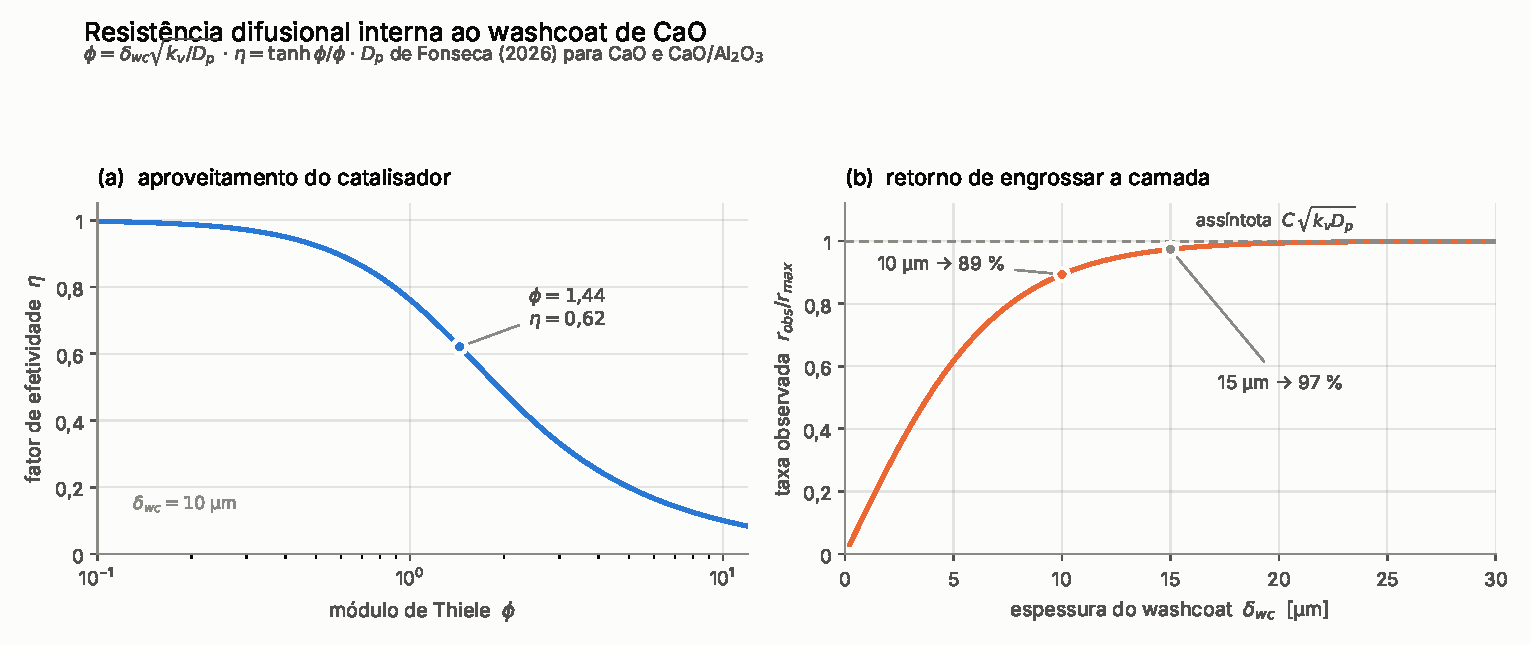
\includegraphics[width=\textwidth]{fig5_thiele_washcoat.pdf}
\caption{Resistência difusional interna ao \textit{washcoat}.
(a)~fator de efetividade em função do módulo de Thiele, com o ponto de operação
adotado neste trabalho; (b)~taxa observada em função da espessura da camada,
normalizada pela assíntota $C\sqrt{k_v D_p}$}
\label{fig:thiele}
\end{figure}

\section{Resistência externa: a camada-limite de concentração}
\label{sec:leveque}

Fora do \textit{washcoat}, o reagente precisa atravessar a camada de fluido que
se empobrece junto à parede. Em escoamento laminar plenamente desenvolvido, com
reação iniciando-se em $x = 0$, a espessura dessa camada é dada pela solução de
Lévêque,

\begin{equation}
\delta_c(x) = \left( \frac{9\,D\,x}{\gamma} \right)^{1/3},
\qquad \gamma = \frac{6\,\bar{u}}{H}
\label{eq:leveque}
\end{equation}

\noindent
em que $\gamma$ é a taxa de cisalhamento junto à parede e $H$ a altura do canal.
A dependência com $x^{1/3}$ é lenta, o que significa que a camada demora a
crescer e que o comprimento necessário para que ela preencha a seção pode ser
muito maior do que a intuição sugere.

Esse comprimento é o comprimento de entrada mássica, estimado por

\begin{equation}
L_e \approx 0{,}05\, D_h\, Re\, Sc
\label{eq:entrada}
\end{equation}

\noindent
com $Re = \rho\,\bar{u}\,D_h/\mu$ e $Sc = \mu/(\rho D)$. O produto $Re\,Sc$ é o
número de Péclet mássico, e é nele que reside a particularidade do sistema
estudado: enquanto o número de Reynolds é pequeno, da ordem de \num{0.2}, o
número de Schmidt de um óleo vegetal ultrapassa \num{1e5}, de modo que o produto
permanece elevado. O Capítulo~\ref{cap:resultados} mostra as consequências
disso para a geometria simulada.

\section{Número de Damköhler e regimes de operação}
\label{sec:damkohler}

A competição entre a reação na parede e o transporte até ela é medida pelo
número de Damköhler de parede, definido como a razão entre a taxa de reação
avaliada na concentração do seio do fluido e o fluxo máximo que o transporte
externo é capaz de sustentar,

\begin{equation}
Da = \frac{r_w(C_b)}{k_m\,C_b}
\label{eq:damkohler}
\end{equation}

\noindent
em que $k_m$ é o coeficiente de transferência de massa. Para reação de primeira
ordem na parede, o balanço em regime permanente entre o que o transporte entrega
e o que a reação consome conduz a uma relação direta entre $Da$ e as
concentrações medidas,

\begin{equation}
\frac{C_w}{C_b} = \frac{1}{1 + Da}
\qquad \Longleftrightarrow \qquad
Da = \frac{C_b}{C_w} - 1
\label{eq:cwcb}
\end{equation}

\noindent
expressão que será empregada no Capítulo~\ref{cap:resultados} para extrair $Da$
diretamente do campo simulado, sem a necessidade de estimar $k_m$ por correlação.

Três regimes são distinguidos. Quando $Da \ll 1$, a reação é lenta em comparação
com o transporte, a concentração junto à parede é praticamente igual à do seio
do fluido e o sistema opera sob controle cinético; nessa situação não há
gradiente apreciável a vencer, e aumentar a área de contato não altera o
desempenho. Quando $Da \gg 1$, a reação consome o reagente assim que ele chega,
a concentração na parede tende a zero e o desempenho passa a ser ditado
exclusivamente pelo transporte. Entre os dois extremos situa-se o regime misto,
no qual as duas resistências são comparáveis e ambas precisam ser consideradas
no projeto.

A classificação do sistema em um desses regimes é, do ponto de vista deste
trabalho, a questão central. É dela que depende a resposta sobre se a geometria
monolítica se justifica para a aplicação pretendida.

Convém registrar que o regime misto não constitui exceção nesta reação. Ao
estudarem a transesterificação de trioleína com metanol sobre ZnAl$_2$O$_4$ em
leito fixo, \textcite{Allain2016} concluíram que a difusão dos triglicerídeos e
a cinética da primeira etapa limitam conjuntamente a conversão global do
sistema. Trata-se de sistema distinto do aqui estudado, com outro catalisador,
outra forma física e outra faixa de temperatura, mas a coexistência das duas
resistências é a mesma situação que o Capítulo~\ref{cap:resultados} identifica
para o canal monolítico com CaO.

\section{Modelagem CFD de reatores de parede catalítica}

A simulação de um canal catalítico requer a solução simultânea das equações de
continuidade e de quantidade de movimento, que fornecem o campo de velocidade, e
das equações de transporte das espécies químicas, acopladas à cinética na
superfície. A reação heterogênea pode ser incorporada de duas formas.

A primeira consiste em discretizar o \textit{washcoat} como uma região porosa
adicional, com suas próprias equações de transporte e um termo fonte
volumétrico. A abordagem é rigorosa, mas impõe custo computacional elevado: a
camada tem espessura da ordem de dezenas de micrômetros, contra milímetros do
canal, e resolvê-la exige malha muito refinada em uma região de pouco interesse
direto.

A segunda trata a reação como condição de contorno de fluxo de espécies na
parede, incorporando a resistência interna por meio do fator de efetividade da
Equação~\eqref{eq:efetividade}. O custo é modesto e a perda de informação é
limitada ao perfil de concentração no interior do poro, que raramente é o objeto
de interesse. Foi esta a abordagem adotada no presente trabalho, e sua
implementação é descrita na Seção~\ref{sec:bc}.

A formulação do transporte multicomponente merece atenção. A lei de Fick, na
qual o fluxo difusivo de cada espécie é proporcional ao seu próprio gradiente,
é a opção padrão dos códigos comerciais e adequada à maior parte das aplicações.
Ela carrega, entretanto, uma restrição pouco discutida: a conservação da massa
total exige que a soma dos fluxos difusivos se anule, condição que só é
satisfeita quando todas as difusividades são iguais entre si. A formulação de
Maxwell-Stefan não tem essa limitação, por satisfazer a restrição de soma por
construção, mas exige difusividades binárias para todos os pares de espécies,
dado raramente disponível para sistemas contendo triglicerídeos. As implicações
dessa escolha para o presente trabalho são tratadas na
Seção~\ref{sec:difusividades}.

\subsection{Aplicações recentes a reatores de biodiesel}

A literatura de simulação aplicada à produção de biodiesel tem se concentrado em
duas frentes, ambas distintas do presente estudo.

A primeira compara configurações de reator quanto ao desempenho global.
\textcite{Omranpour2024} modelaram a transesterificação de óleo de canola com
metanol sobre ácido tungstofosfórico sólido, confrontando um reator de leito
fixo com um reator de membrana de leito empacotado. O modelo é bidimensional e
heterogêneo, resolvido numericamente. Nas melhores condições identificadas,
\SI{180}{\celsius}, razão molar de \num{15}:\num{1} e vazão de alimentação de
\SI{0.5}{\milli\liter\per\minute}, a conversão de \SI{99.94}{\percent} foi
atingida com \SI{86}{\centi\meter} de reator de membrana contra
\SI{2.75}{\meter} de leito fixo --- uma redução de comprimento por um fator
próximo de três para a mesma conversão. O consumo energético estimado para uma
planta de \SI{8000}{\tonne} por ano resultou em \SI{1313}{\kilo\watt} contra
\SI{1352}{\kilo\watt}, diferença bem menor que a de comprimento.

Esse resultado é instrutivo para o presente trabalho por tratar justamente da
relação entre comprimento de reator e conversão, que o
Capítulo~\ref{cap:resultados} identifica como a limitação dominante do canal
monolítico simulado.

A segunda frente trata de reatores de microcanal. \textcite{Laziz2020}
reportaram conversão de \SI{98.6}{\percent} em \SI{40}{\second} de reação à
temperatura ambiente, em microcanal de \SI{690}{\micro\meter} de diâmetro
alimentado por junção em T, empregando óleo de palma e hidróxido de potássio.
A simulação tridimensional com modelo de volume de fluido revelou uma estrutura
de recirculação toroidal no interior do pistão de metanol, à qual os autores
atribuem a intensificação da transferência de massa através da interface
líquido-líquido. \textcite{Subramaniam2024} revisaram o estado da arte dessas
tecnologias, destacando a razão área/volume elevada, a intensificação da mistura
por geometria de canal, micromisturadores e padrões de escoamento em pistão, e o
aquecimento por irradiação de micro-ondas como vias de intensificação.

A aproximação entre microcanais e monólitos merece comentário, por não ser
imediata. Ambas as configurações reduzem a distância que o reagente percorre até
onde a reação ocorre, mas o fazem em regimes distintos. No trabalho de
\textcite{Laziz2020} o catalisador é hidróxido de potássio dissolvido, isto é, a
catálise é homogênea, e a resistência a vencer é a transferência de massa
através da interface entre duas fases imiscíveis; o que se intensifica é a
mistura. No monólito de parede catalítica a fase é única e a reação é
heterogênea, de modo que a resistência a vencer é o transporte difusivo até uma
superfície sólida. As conclusões de uma literatura não se transferem
automaticamente à outra, e a comparação precisa ser feita pelos grupos
adimensionais, e não pela semelhança geométrica.

\chapter{Modelagem Matemática e Métodos Numéricos}
\label{cap:modelagem}

Este capítulo descreve o modelo construído para representar um canal do reator
monolítico, as hipóteses que o sustentam, a forma como a reação heterogênea foi
incorporada e os procedimentos adotados para verificar a solução numérica. As
simulações foram conduzidas no código comercial Simcenter STAR-CCM+
\parencite{StarCCMUserGuide}.

\section{Domínio e hipóteses}

O domínio computacional representa um único canal do monólito, tratado como
representativo do feixe pelas razões discutidas no
Capítulo~\ref{cap:revisao}. A Figura~\ref{fig:dominio} resume sua geometria e
as condições de contorno impostas.

Adotou-se um paralelepípedo de \SI{50}{\milli\meter} de comprimento por
\SI{1.1}{\milli\meter} de altura e \SI{50}{\micro\meter} de espessura. Nas duas
faces normais à direção de menor dimensão impôs-se condição de simetria, e a
malha contém uma única célula nessa direção. O domínio comporta-se, assim, como
um canal plano bidimensional, embora a formulação do solver permaneça
tridimensional. O artifício evita as restrições que a formulação bidimensional
estrita impõe à especificação de condições de contorno de espécies no código
empregado, sem o custo de uma terceira direção efetivamente discretizada.

A parede superior é catalítica e a inferior é tratada como parede lisa inerte.
A escolha merece registro por ser conservadora: um canal real de monólito tem
todas as paredes recobertas, de modo que a razão entre área catalítica e volume
do presente domínio é metade da de um canal plano com ambas as paredes ativas,
e um oitavo da do canal quadrado das peças efetivamente disponíveis no
laboratório. A comparação entre as duas geometrias é retomada na
Seção~\ref{sec:geomreal}; o que importa aqui é que o regime de operação
determinado no Capítulo~\ref{cap:resultados} não depende dessa razão, por ser
estabelecido localmente na parede.

\begin{figure}[htb]
\centering
\begin{tikzpicture}[x=0.78cm, y=0.78cm,
    >={Latex[length=4pt,width=3pt]},
    cota/.style={tinta3viz, line width=0.5pt, |<->|,
                 >={Latex[length=3.5pt,width=2.8pt]}},
    aux/.style={tinta3viz, line width=0.35pt, dash pattern=on 2pt off 1.5pt}]

% ---------- camada-limite de concentração (sombreado sob a parede ativa) ----
\fill[azulviz!12]
  plot[domain=0.0001:12, samples=80] ({\x}, {2.40 - 0.55*((\x/12)^(1/3))})
  -- (12,2.40) -- (0,2.40) -- cycle;
\draw[azulviz!55, line width=0.6pt]
  plot[domain=0.0001:12, samples=80] ({\x}, {2.40 - 0.55*((\x/12)^(1/3))});
\node[azulviz!75!black, font=\footnotesize, anchor=north east] at (11.7,1.70)
  {$\delta_c(x)$};

% ---------- canal -----------------------------------------------------------
\draw[tintaviz, line width=0.8pt] (0,0) rectangle (12,2.40);

% ---------- parede catalítica (superior) ------------------------------------
\fill[pattern=north east lines, pattern color=laranjaviz!65]
  (0,2.40) rectangle (12,2.70);
\draw[laranjaviz!85!black, line width=0.9pt] (0,2.40) -- (12,2.40);
\draw[laranjaviz!85!black, line width=0.9pt] (0,2.70) -- (12,2.70);
\node[font=\footnotesize, tintaviz, anchor=south] at (6,3.18)
  {parede catalítica};
\draw[cota] (12.35,2.40) -- (12.35,2.70);
\node[font=\footnotesize, tintaviz, anchor=west] at (12.5,2.55)
  {$\delta_{wc} = 10$ µm};

% ---------- parede inerte (inferior) ----------------------------------------
\fill[tinta3viz!45] (0,-0.30) rectangle (12,0);
\draw[tintaviz, line width=0.8pt] (0,-0.30) rectangle (12,0);
\node[font=\footnotesize, tintaviz, anchor=north] at (6,-0.46)
  {parede lisa inerte};

% ---------- perfil de velocidade na entrada ---------------------------------
\draw[aux] (-2.05,0) -- (-2.05,2.40);
\draw[azulviz, line width=0.9pt]
  plot[domain=0:2.40, samples=60] ({-2.05 + 1.55*4*(\x/2.40)*(1-\x/2.40)}, {\x});
\foreach \y in {0.3,0.6,0.9,1.2,1.5,1.8,2.1}{
  \draw[->, azulviz, line width=0.5pt]
    (-2.05,{\y}) -- ({-2.05 + 1.55*4*(\y/2.40)*(1-\y/2.40)}, {\y});}
\node[azulviz, font=\footnotesize, anchor=east] at (-2.2,1.20) {$\bar{u}$};

% ---------- fluxo de espécies na parede -------------------------------------
\foreach \x in {2.4,5.0,7.6}{
  \draw[->, laranjaviz!85!black, line width=0.6pt] ({\x},1.82) -- ({\x},2.32);
  \draw[->, laranjaviz!85!black, line width=0.6pt] ({\x+0.55},2.32) -- ({\x+0.55},1.82);}
\node[laranjaviz!85!black, font=\footnotesize, anchor=west] at (8.55,2.07) {$J_i$};

% ---------- rótulos de fronteira --------------------------------------------
\node[font=\footnotesize, tintaviz, anchor=north] at (0,-0.46)  {entrada};
\node[font=\footnotesize, tintaviz, anchor=north] at (12,-0.46) {saída};

% ---------- cotas ------------------------------------------------------------
\draw[aux] (0,-0.46) -- (0,-1.45);
\draw[aux] (12,-0.46) -- (12,-1.45);
\draw[cota] (0,-1.30) -- (12,-1.30);
\node[font=\footnotesize, tintaviz, fill=white, inner sep=1.5pt]
  at (6,-1.30) {$L = 50$ mm};

\draw[aux] (12,0)    -- (13.05,0);
\draw[aux] (12,2.40) -- (13.05,2.40);
\draw[cota] (12.90,0) -- (12.90,2.40);
\node[font=\footnotesize, tintaviz, anchor=west] at (13.05,1.20)
  {$H = 1{,}1$ mm};

\end{tikzpicture}
\caption{Representação esquemática do domínio computacional, fora de escala.
O escoamento entra à esquerda com perfil de Poiseuille plenamente desenvolvido;
a reação heterogênea é imposta como fluxo de espécies $J_i$ na parede superior,
recoberta pelo \textit{washcoat}. O sombreado indica a camada-limite de
concentração que se desenvolve a partir da entrada. As duas faces normais a
$z$, afastadas de \SI{50}{\micro\meter} e discretizadas com uma única célula,
recebem condição de simetria}
\label{fig:dominio}
\end{figure}

As hipóteses adotadas são as seguintes:

\begin{enumerate}
\itemsep2pt
\item escoamento laminar, incompressível e isotérmico a \SI{65}{\celsius};
\item propriedades físicas constantes, de modo que o campo de velocidade fica
      desacoplado do campo de concentrações;
\item reação restrita à superfície da parede recoberta, sem discretização da
      camada de \textit{washcoat};
\item transporte difusivo descrito pela lei de Fick com difusividades efetivas
      iguais para todas as espécies, pelas razões expostas na
      Seção~\ref{sec:difusividades};
\item cinética irreversível de pseudo-primeira ordem no triglicerídeo, com
      metanol em excesso.
\end{enumerate}

A primeira hipótese se justifica pelo número de Reynolds do escoamento, da ordem
de \num{0.2}, e pela condução do processo em banho termostatizado. A segunda
decorre das faixas estreitas de composição percorridas pelo meio reacional ao
longo do canal, dada a conversão por passe baixa que se verifica no
Capítulo~\ref{cap:resultados}. A quinta é sustentada pela razão molar de
\num{4}:\num{1} entre metanol e óleo, que mantém a concentração de álcool
praticamente inalterada ao longo da reação, e pela baixa conversão por passe,
condição sob a qual \textcite{Ezzati2021} demonstram que a aproximação de
pseudo-primeira ordem é acurada.

\section{Equações governantes}

Com massa específica e viscosidade constantes, a continuidade e a quantidade de
movimento assumem a forma

\begin{align}
\nabla \cdot \mathbf{u} &= 0 \label{eq:continuidade}\\[4pt]
\rho \left( \frac{\partial \mathbf{u}}{\partial t} + \mathbf{u} \cdot \nabla \mathbf{u} \right)
&= -\nabla p + \mu \nabla^2 \mathbf{u} \label{eq:momento}
\end{align}

O transporte das $N = 4$ espécies consideradas, a saber TG, MeOH, FAME e GL, é
descrito por

\begin{equation}
\frac{\partial (\rho Y_i)}{\partial t} + \nabla \cdot (\rho\, \mathbf{u}\, Y_i)
= \nabla \cdot \left( \rho\, D_i\, \nabla Y_i \right),
\qquad i = 1, \ldots, N
\label{eq:especies}
\end{equation}

\noindent
sem termo fonte volumétrico, uma vez que toda a reação é imposta pela condição
de contorno de parede. O solver garante $\sum_i Y_i = 1$ por normalização, o que
tem implicações discutidas na Seção~\ref{sec:difusividades}.

\section{Cinética e condição de contorno catalítica}
\label{sec:bc}

A taxa de reação por área de parede foi escrita como de primeira ordem aparente
no triglicerídeo, corrigida pelo fator de efetividade que contabiliza a
resistência interna ao \textit{washcoat}:

\begin{equation}
r_w = \eta\, k_{cat}\, w\, C_{TG}\big|_{\text{parede}}
\label{eq:rw}
\end{equation}

\noindent
em que $C_{TG} = \rho\, Y_{TG}/M_{TG}$ é a concentração molar de triglicerídeo
avaliada junto à superfície, $k_{cat}$ a constante cinética por massa de
catalisador e $w$ a massa de catalisador por área de parede, dada por

\begin{equation}
w = \rho_{wc}\, \delta_{wc}
\label{eq:w}
\end{equation}

A constante cinética foi tomada de \textcite{Melo2023}, que a determinou para
CaO suportado em biochar na metanólise de óleo de soja a \SI{65}{\celsius}:

\begin{equation}
k_{cat} = \SI{5.302e-5}{\meter\cubed\per\kilogram\per\second}
\end{equation}

Na ausência de medidas da camada depositada, adotaram-se
$\rho_{wc} = \SI{1700}{\kilogram\per\meter\cubed}$ e
$\delta_{wc} = \SI{10}{\micro\meter}$, o que resulta em
$w = \SI{1.70e-2}{\kilogram\per\meter\squared}$. Convém registrar que a taxa da
Equação~\eqref{eq:rw} é linear no produto $\rho_{wc}\,\delta_{wc}$, de modo que
a caracterização experimental dessas duas grandezas é a medida de maior retorno
imediato para a acurácia do modelo.

\pendente{substituir $\rho_{wc}$ e $\delta_{wc}$ pelos valores medidos assim que
as caracterizações do \textit{washcoat} estiverem concluídas}

Os fluxos mássicos de cada espécie na parede decorrem da estequiometria da
Equação~\eqref{eq:global}, com sinal negativo para os reagentes e positivo para
os produtos:

\begin{align}
J_{TG}   &= -M_{TG}\, r_w        &&= -872{,}00\, r_w \label{eq:fluxTG}\\
J_{MeOH} &= -3\,M_{MeOH}\, r_w   &&= -\phantom{0}96{,}12\, r_w \label{eq:fluxMeOH}\\
J_{FAME} &= +3\,M_{FAME}\, r_w   &&= +876{,}00\, r_w \label{eq:fluxFAME}\\
J_{GL}   &= +M_{GL}\, r_w        &&= +\phantom{0}92{,}09\, r_w \label{eq:fluxGL}
\end{align}

A soma dos quatro coeficientes vale $-0{,}03$ quilogramas por quilomol de
triglicerídeo consumido, ou \num{3e-5} da massa envolvida, resíduo que decorre
apenas do arredondamento das massas molares. Essa verificação não é
dispensável: coeficientes que não se cancelam injetam ou removem massa total na
parede, e o solver redistribui o desvio pela normalização de $\sum_i Y_i$,
produzindo um erro que não se manifesta em nenhum dos indicadores usuais de
convergência.

\section{Resistência interna ao \textit{washcoat}}

A difusão no interior da camada porosa foi tratada pelo módulo de Thiele para
placa plana, Equações~\eqref{eq:thiele} e~\eqref{eq:efetividade}. Com a
difusividade efetiva no poro tomada da faixa reportada por
\textcite{Fonseca2026} para CaO e CaO/Al$_2$O$_3$, e com
$\delta_{wc} = \SI{10}{\micro\meter}$, obtém-se

\begin{equation}
\phi = 1{,}44
\qquad \Longrightarrow \qquad
\eta = 0{,}62
\end{equation}

Ou seja, pouco menos de \SI{40}{\percent} da atividade nominal do catalisador
depositado é perdida por limitação difusional interna já nessa espessura.

O comportamento da taxa observada com a espessura da camada merece ser
explicitado, por ter consequência direta sobre o procedimento de impregnação.
Substituindo-se a Equação~\eqref{eq:efetividade} na taxa por área de parede,

\begin{equation}
r_{obs} = \eta\, k_v\, \delta_{wc}\, C
        = C \sqrt{k_v D_p}\, \tanh \phi
\label{eq:saturacao}
\end{equation}

\noindent
de modo que a taxa não passa por máximo: ela cresce monotonicamente e satura em
$C\sqrt{k_v D_p}$, valor que independe da espessura depositada. O que se perde
ao engrossar a camada não é taxa, e sim material, que passa a ser depositado sem
contribuir.

Com a calibração adotada, $\phi = \num{1.44}$ a \SI{10}{\micro\meter}
corresponde a $\tanh\phi = \num{0.894}$, ou seja, \SI{89}{\percent} da taxa
máxima alcançável. Aos \SI{15}{\micro\meter} chega-se a \SI{97}{\percent}, e
aos \SI{20}{\micro\meter} a \SI{99}{\percent}. A faixa de trabalho
recomendada é, portanto, de \SIrange{10}{15}{\micro\meter}: abaixo disso
perde-se taxa de forma apreciável, e acima disso acrescenta-se catalisador cujo
retorno é inferior a três pontos percentuais. Essa recomendação foi repassada à
equipe responsável pelas impregnações.

\section{Propriedades físicas e difusividades}
\label{sec:difusividades}

As propriedades adotadas estão reunidas na Tabela~\ref{tab:propriedades}. A
composição de entrada corresponde à razão molar de \num{4}:\num{1} entre metanol
e triglicerídeo,

\begin{equation}
Y_{TG} = \frac{872}{872 + 4 \times 32{,}04} = 0{,}8719,
\qquad Y_{MeOH} = 0{,}1281
\label{eq:composicao}
\end{equation}

\noindent
escolha que merece justificativa, por divergir da razão de \num{6}:\num{1} usual
na prática industrial. A constante cinética adotada na Equação~\eqref{eq:rw} foi
determinada por \textcite{Melo2023} em ensaios conduzidos com
\SI{1}{\percent} em massa de CaO, razão molar metanol:óleo de \num{4}:\num{1} e
\SI{65}{\celsius}. Alimentar o modelo com razão diferente daquela em que a
cinética foi ajustada introduziria inconsistência entre o parâmetro e a condição
de contorno, ainda que o efeito numérico seja pequeno: por se tratar de cinética
de pseudo-primeira ordem, tanto o número de Damköhler quanto a conversão
fracionária são razões e independem, em primeira aproximação, do valor absoluto
da concentração de entrada. Essa independência foi verificada por simulação, e
os valores medidos constam da Seção~\ref{sec:invariancia}.

A escolha tem ainda um benefício colateral. Segundo as medidas de solubilidade
de \textcite{Firth2014}, a \SI{65}{\celsius} o óleo vegetal dissolve metanol até
a razão de \num{3}:\num{1}; uma alimentação de \num{4}:\num{1} está, portanto,
mais próxima do limite de miscibilidade do que uma de \num{6}:\num{1}, o que
atenua, sem eliminar, a fragilidade discutida na
Seção~\ref{sec:limitacoes}.

\begin{table}[htb]
\centering
\caption{Propriedades físicas e condições operacionais adotadas}
\label{tab:propriedades}
\begin{tabular}{l c c l}
\toprule
Propriedade & Símbolo & Valor & Unidade \\
\midrule
Massa específica do meio      & $\rho$      & \num{868}      & \si{\kilogram\per\meter\cubed} \\
Viscosidade dinâmica          & $\mu$       & \num{1.05e-2}  & \si{\pascal\second} \\
Difusividade efetiva          & $D_i$       & \num{7.0e-11}  & \si{\meter\squared\per\second} \\
Temperatura                   & $T$         & \num{65}       & \si{\celsius} \\
Velocidade média              & $\bar{u}$   & \num{1.0e-3}   & \si{\meter\per\second} \\
Altura do canal               & $H$         & \num{1.1}      & \si{\milli\meter} \\
Comprimento do canal          & $L$         & \num{50}       & \si{\milli\meter} \\
Massa específica do washcoat  & $\rho_{wc}$ & \num{1700}     & \si{\kilogram\per\meter\cubed} \\
Espessura do washcoat         & $\delta_{wc}$ & \num{10}     & \si{\micro\meter} \\
\bottomrule
\end{tabular}
\end{table}

A igualdade imposta entre as difusividades das quatro espécies não é uma
simplificação cosmética, e merece ser justificada com algum cuidado. Na
formulação de Fick, o fluxo difusivo de cada espécie é escrito como
$\mathbf{j}_i = -\rho D_i \nabla Y_i$. A conservação da massa total exige que a
soma desses fluxos se anule,

\begin{equation}
\sum_i \mathbf{j}_i = -\rho \sum_i D_i \nabla Y_i = 0
\label{eq:somafluxos}
\end{equation}

\noindent
e, como $\sum_i Y_i = 1$ implica $\sum_i \nabla Y_i = 0$, a
Equação~\eqref{eq:somafluxos} só é satisfeita identicamente quando todas as
difusividades forem iguais entre si. Com difusividades distintas, a soma das
frações mássicas deriva da unidade a cada passo de tempo, e o solver a
restabelece por normalização, distribuindo o desvio proporcionalmente a $Y_i$.
O erro recai, portanto, quase integralmente sobre a espécie majoritária.

No sistema estudado o triglicerídeo responde por \SI{82}{\percent} da massa e o
metanol possui difusividade cerca de noventa vezes maior, dada a diferença de
tamanho molecular. Nessas condições, simulações preliminares conduzidas com
difusividades individuais apresentaram erro de \SI{374}{\percent} no balanço de
massa do triglicerídeo, sem que resíduos, somas de frações mássicas ou fluxos de
parede indicassem qualquer anormalidade. A adoção de um valor efetivo único,
$D_i = \SI{7.0e-11}{\meter\squared\per\second}$, reduziu esse erro a
\SI{0.013}{\percent}.

A perda física associada à simplificação é real e deve ser declarada: a
seletividade difusional entre espécies é suprimida. No presente caso a
simplificação é defensável, pois o reagente limitante é o triglicerídeo, o
metanol se encontra em excesso e o objeto de interesse é a competição entre
cinética de parede e transporte externo do próprio triglicerídeo. Caso a
seletividade entre espécies venha a se tornar relevante, a alternativa correta é
a formulação de Maxwell-Stefan, condicionada à obtenção de difusividades
binárias para todos os pares.

\section{Malha}

Empregou-se malha do tipo \textit{trimmer} com dimensão de base de
\SI{50}{\micro\meter}, igual à espessura do domínio na direção de simetria, o
que força uma única célula nessa direção. Junto às duas paredes foram geradas
camadas prismáticas com os parâmetros da Tabela~\ref{tab:malha}, resultando em
\num{88000} células.

\begin{table}[htb]
\centering
\caption{Parâmetros da malha}
\label{tab:malha}
\begin{tabular}{l c}
\toprule
Parâmetro & Valor \\
\midrule
Dimensão de base                      & \SI{50}{\micro\meter} \\
Número de camadas prismáticas         & \num{15} \\
Espessura total das camadas           & \SI{200}{\micro\meter} \\
Razão de crescimento                  & \num{1.2} \\
Espessura da primeira camada          & \SI{2.8}{\micro\meter} \\
Número total de células               & \num{88000} \\
\bottomrule
\end{tabular}
\end{table}

O refino junto à parede não é opcional neste problema. Com $Sc = \num{1.7e5}$, o
gradiente de fração mássica na superfície catalítica atinge

\begin{equation}
\left. \frac{\partial Y}{\partial n} \right|_{\text{parede}}
= \frac{J}{\rho D} \approx \SI{3.9e3}{\per\meter}
\end{equation}

\noindent
o que corresponde a uma variação de $\Delta Y \approx 0{,}20$ ao longo de uma
célula de \SI{50}{\micro\meter}, ou \SI{40}{\percent} do valor de parede. Sem as
camadas prismáticas, o valor de face lido pela condição de contorno é uma
extrapolação sem significado físico, e o balanço global de massa apresenta
desvios de dezenas de pontos percentuais já nos primeiros segundos de simulação.

\section{Discretização e marcha temporal}

Adotou-se formulação implícita transiente com \num{30} iterações internas por
passo de tempo. O erro de discretização temporal escala linearmente com o passo,
dada a ordem do esquema de Euler implícito; mediu-se contribuição de
aproximadamente \num{4.5} pontos percentuais no balanço de massa com
$\Delta t = \SI{0.05}{\second}$, reduzida a cerca de \num{0.45} ponto com
$\Delta t = \SI{5e-3}{\second}$. A marcha foi conduzida com
$\Delta t = \SI{5e-3}{\second}$ na partida e $\Delta t = \SI{2e-2}{\second}$ no
trecho longo, com refinamento final antes da extração dos resultados.

\section{Procedimento de verificação}
\label{sec:verificacao}

A verificação apoia-se em três testes independentes, todos necessários. A
experiência acumulada ao longo do trabalho mostrou que nenhum deles,
isoladamente, é suficiente para detectar os modos de falha encontrados.

O primeiro é a \textbf{consistência estequiométrica}. A razão entre as taxas de
acúmulo de FAME e de consumo de triglicerídeo no domínio deve igualar a razão
mássica estequiométrica,

\begin{equation}
\frac{\mathrm{d}M_{FAME}/\mathrm{d}t}{\mathrm{d}M_{TG}/\mathrm{d}t}
= \frac{876}{872} = 1{,}004587
\label{eq:esteq}
\end{equation}

\noindent
restrição exata, independente da malha, do passo de tempo e do estado de
convergência. É o único teste que flagra a violação de conservação descrita na
Seção~\ref{sec:difusividades}.

O segundo é a \textbf{independência de malha}, verificada pela reprodução do
resultado central em configurações distintas de discretização.

O terceiro é o \textbf{balanço global de massa} por espécie, escrito como

\begin{equation}
\frac{\mathrm{d}}{\mathrm{d}t} \int_V \rho\, Y_i\, \mathrm{d}V
= \dot{m}\left( Y_{i,\text{ent}} - Y_{i,\text{sai}} \right) + \oint_{A_p} J_i\, \mathrm{d}A
\label{eq:balanco}
\end{equation}

\noindent
com todos os termos medidos de forma independente. É o teste mais trabalhoso e o
mais importante, pois resíduos, somas de frações mássicas e fluxos de parede
podem apresentar-se simultaneamente corretos enquanto o balanço falha por ordens
de grandeza.

Uma observação de ordem prática, decorrente da experiência deste trabalho, deve
acompanhar a Equação~\eqref{eq:balanco}. O termo convectivo não pode ser
avaliado pela média de fração mássica ponderada por vazão na fronteira de saída,
pelas razões documentadas na Seção~\ref{sec:reports}. Em seu lugar, emprega-se a
integração numérica de um perfil transversal medido por sonda de linha, ou
calcula-se a conversão diretamente pela integral do fluxo de parede.

\section{Limitações declaradas do modelo}
\label{sec:limitacoes}

Três hipóteses do modelo merecem ser explicitadas como limitações, por terem
sido confrontadas com dados experimentais da literatura durante a redação deste
texto. São enumeradas a seguir em ordem decrescente de gravidade.

\begin{enumerate}
\itemsep10pt

\item \textbf{Hipótese de fase única.}

O modelo trata o meio reacional como uma única fase líquida homogênea. As
medidas de solubilidade de \textcite{Firth2014} indicam, porém, que a
\SI{65}{\celsius} o óleo vegetal dissolve metanol apenas até a razão molar de
\num{3}:\num{1}, ao passo que a alimentação aqui adotada é de \num{4}:\num{1}.
Na entrada do canal, portanto, parte do álcool pode constituir fase separada, e
o sistema seria bifásico.

O quadro é, na verdade, mais desfavorável do que essa comparação sugere.
\textcite{Muller2019} registra que a mistura de óleo e metanol só se torna
homogênea a partir de \SIrange{15}{20}{\percent} de conversão, patamar muito
acima da conversão por passe de \SI{1.4}{\percent} obtida neste trabalho. O
canal simulado operaria, assim, em regime bifásico em toda a sua extensão.

Dois atenuantes se aplicam, e convém dimensioná-los com honestidade. O primeiro
é que o éster formado atua como cossolvente, de modo que a miscibilidade aumenta
à medida que a reação avança; isso importa pouco em um único passe, mas passa a
importar em configurações com reciclo ou com várias peças em série, nas quais a
conversão acumulada pode ultrapassar aquele patamar. O segundo é que o reagente
limitante e o objeto de interesse deste trabalho é o triglicerídeo, cuja
concentração na fase oleosa é a que governa a taxa de parede, ao passo que o
metanol, estando em excesso, não limita.

Ainda assim, esta é a hipótese mais frágil do modelo, e convém delimitar com
precisão o que ele descreve. O que o modelo resolve com rigor é o transporte de
triglicerídeo no interior da fase oleosa até a parede catalítica. A
disponibilidade de metanol nessa parede, governada pela transferência entre
fases, fica fora de seu alcance. A verificação experimental dessa hipótese
consta das atividades previstas no Capítulo~\ref{cap:cronograma}, e a extensão
do modelo a duas fases é a principal direção de trabalho futuro que dela
decorre.

\item \textbf{Propriedades físicas constantes.}

A massa específica e a viscosidade foram tomadas como constantes.
\textcite{Firth2014} atribui à viscosidade elevada do meio rico em
triglicerídeo uma fase inicial de inibição da reação, o que indicaria
dependência da taxa com a composição.

No presente caso a hipótese é defensável precisamente pelo resultado obtido:
com conversão por passe de \SI{1.4}{\percent}, a composição do meio percorre
faixa estreita ao longo do canal, e as propriedades não chegam a variar de forma
apreciável. A hipótese deixaria de valer em configurações de conversão elevada.

\item \textbf{Cinética irreversível.}

A reação global é reversível, e o modelo a trata como irreversível. A
aproximação é válida enquanto a composição estiver longe do equilíbrio,
condição também assegurada pela baixa conversão por passe.

\end{enumerate}

As três limitações têm a mesma origem e o mesmo remédio. Todas decorrem de se
extrapolar um modelo construído para conversão baixa, e todas serão reexaminadas
quando a calibração experimental prevista no Capítulo~\ref{cap:cronograma}
fornecer dados em faixas mais amplas.

\chapter{Resultados Preliminares}
\label{cap:resultados}

Reúnem-se neste capítulo os resultados já obtidos com o modelo descrito no
Capítulo~\ref{cap:modelagem}.

Os resultados aqui reunidos foram obtidos em duas corridas independentes, com
alimentações de razão molar \num{4}:\num{1} e \num{6}:\num{1}. A primeira
corresponde à condição em que \textcite{Melo2023} determinou a constante
cinética e é, por isso, a adotada no Capítulo~\ref{cap:modelagem}; a segunda foi
conduzida antes dessa constatação. A comparação entre as duas, apresentada na
Seção~\ref{sec:invariancia}, constitui um teste de verificação adicional, e os
valores reportados adiante são comuns a ambas.

A exposição segue a ordem em que os testes foram
conduzidos: primeiro a verificação do campo de velocidade, depois a dos
balanços de massa, e por fim a caracterização do regime de operação, que
constitui o resultado central do trabalho até o momento.

\section{Verificação hidrodinâmica}

O campo de velocidade foi verificado contra a solução analítica de Poiseuille
para canal plano,

\begin{equation}
u(y) = 6\,\bar{u}\,\frac{y}{H}\left(1 - \frac{y}{H}\right)
\label{eq:poiseuille}
\end{equation}

\noindent
por meio de um perfil transversal medido a \SI{49}{\milli\meter} da entrada,
apresentado na Figura~\ref{fig:poiseuille}.

\begin{figure}[htb]
\centering
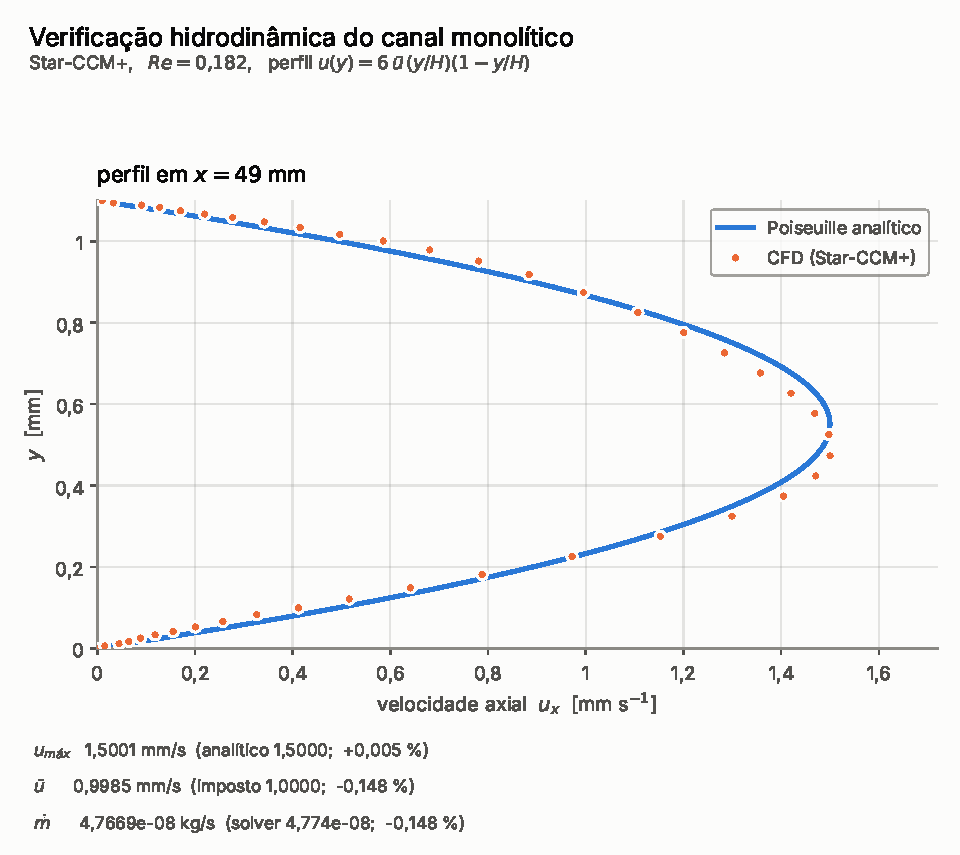
\includegraphics[width=0.74\textwidth]{fig6_poiseuille_fase3.pdf}
\caption{Perfil transversal de velocidade axial em $x = \SI{49}{\milli\meter}$,
comparado à solução analítica de Poiseuille para canal plano}
\label{fig:poiseuille}
\end{figure}

A concordância é satisfatória nas três grandezas integrais verificadas. A
velocidade máxima medida vale \SI{1.5001}{\milli\meter\per\second}, contra
$1{,}5\,\bar{u} = \SI{1.5000}{\milli\meter\per\second}$ previstos, diferença de
\SI{0.005}{\percent}. A integração do perfil fornece velocidade média de
\SI{0.9985}{\milli\meter\per\second}, \SI{0.15}{\percent} abaixo do valor
imposto na entrada, e vazão mássica de
\SI{4.767e-8}{\kilogram\per\second}, também \SI{0.15}{\percent} abaixo da
registrada pelo solver nas duas fronteiras.

Ponto a ponto, os valores junto às paredes apresentam dispersão maior, da ordem
de \SI{20}{\percent} nas primeiras células. O exame dessa dispersão mostra que
ela corresponde a um deslocamento aparente de aproximadamente
\SI{9}{\micro\meter} entre a coordenada reportada pela sonda de linha e a
posição física das células da malha, e não a um erro da solução: um ajuste
parabólico aos valores de célula fornece raízes em \SI{7.9}{\micro\meter} e
\SI{1109.5}{\micro\meter}, ou seja, altura de canal de
\SI{1101.6}{\micro\meter} contra os \SI{1100}{\micro\meter} nominais. Como as
três grandezas integrais concordam dentro de \SI{0.15}{\percent}, considera-se
o campo de velocidade verificado.

A perda de carga calculada foi de \SI{5.463}{\pascal}, contra
\SI{5.207}{\pascal} da solução de Hagen-Poiseuille,
$\Delta P = 12\,\mu\,\bar{u}\,L/H^2$, diferença de \SI{4.9}{\percent}. Essa
discrepância convive com a concordância de \SI{0.15}{\percent} nas grandezas
cinemáticas, e não compromete o transporte de espécies, que depende do campo de
velocidade e não da pressão.

Registre-se, por fim, uma observação de caráter prático a respeito da perda de
carga. Ela não constitui indicador de qualidade de malha neste problema: a
solução plenamente desenvolvida é um perfil parabólico, que um esquema de
volumes finitos de segunda ordem integra exatamente em qualquer discretização.
Obteve-se, de fato, valor idêntico até a sétima casa decimal em malhas com e sem
camadas prismáticas. O refino junto à parede, indispensável ao transporte de
espécies pelas razões da Seção~\ref{sec:verificacao}, é invisível a esse teste.

\section{Conservação de massa e independência de malha}

A consistência estequiométrica, definida pela Equação~\eqref{eq:esteq}, foi
monitorada ao longo de todas as simulações. Os valores medidos situaram-se entre
\num{1.00455} e \num{1.00462}, contra o valor teórico de \num{1.004587}, o que
representa concordância de \SI{0.009}{\percent}. A estabilidade dessa razão ao
longo de toda a marcha temporal, desde os primeiros décimos de segundo até o
regime permanente, constitui a evidência mais direta de que o transporte de
espécies conserva massa no modelo.

A independência de malha foi avaliada por meio da reprodução do resultado
central em duas configurações distintas, cujos parâmetros e resultados estão
reunidos na Tabela~\ref{tab:malhas}. As duas configurações diferem não apenas na
discretização, mas também na composição de alimentação, e ainda assim
concordam dentro de \SI{2}{\percent}.

\begin{table}[htb]
\centering
\caption{Independência de malha e de composição de alimentação}
\label{tab:malhas}
\begin{tabular}{l c c c c}
\toprule
Configuração & Primeira célula & Alimentação & $C_w/C_b$ & $Da$ \\
\midrule
Sem camadas prismáticas & \SI{50}{\micro\meter}  & \num{4}:\num{1} molar & \num{0.578} & \num{0.730} \\
Com camadas prismáticas & \SI{2.8}{\micro\meter} & \num{6}:\num{1} molar & \num{0.574} & \num{0.743} \\
\bottomrule
\end{tabular}
\end{table}

\subsection{Invariância com a composição de alimentação}
\label{sec:invariancia}

A Seção~\ref{sec:difusividades} argumenta que, por se tratar de cinética de
pseudo-primeira ordem, tanto o número de Damköhler quanto a conversão
fracionária são razões e independem, em primeira aproximação, do valor absoluto
da concentração de entrada. A disponibilidade de duas corridas convergidas com
alimentações distintas permite submeter esse argumento a teste.

A grandeza adequada para a comparação é o empobrecimento relativo do domínio em
regime permanente, $(Y_{in} - Y_{bulk})/Y_{in}$, que deve ser idêntico nas duas
corridas caso a invariância se verifique. A Tabela~\ref{tab:invariancia} reúne
os valores medidos.

\begin{table}[htb]
\centering
\caption{Empobrecimento relativo do domínio em regime permanente para duas
composições de alimentação}
\label{tab:invariancia}
\begin{tabular}{c c c c}
\toprule
Alimentação & $Y_{TG}$ na entrada & $Y_{TG}$ no domínio & Queda relativa \\
\midrule
\num{4}:\num{1} molar & \num{0.8719} & \num{0.848043} & \SI{2.7363}{\percent} \\
\num{6}:\num{1} molar & \num{0.8194} & \num{0.796979} & \SI{2.7363}{\percent} \\
\bottomrule
\end{tabular}
\end{table}

As duas corridas concordam em quatro casas decimais, com discrepância de
\SI{0.001}{\percent}. A invariância prevista pelo argumento cinético verifica-se,
portanto, de forma essencialmente exata, e os valores de $Da$ e de $X_{TG}$
reportados nas seções seguintes valem para ambas as composições.

Registre-se que a concordância é mais estreita do que a de qualquer outro teste
de verificação aplicado ao modelo, incluindo a independência de malha. Isso é
esperado: trata-se da mesma malha e do mesmo conjunto de equações, diferindo
apenas o valor numérico de uma condição de contorno sobre a qual a solução, por
construção, deveria ser linear.

O balanço global de massa, Equação~\eqref{eq:balanco}, foi verificado em regime
permanente. A marcha foi conduzida até \SI{303}{\second}, instante em que o
inventário do domínio deixa de evoluir:

\begin{equation}
\frac{\mathrm{d}M_{TG}}{\mathrm{d}t} = \SI{-2.21e-14}{\kilogram\per\second}
= \SI{0.004}{\percent} \text{ do fluxo de parede}
\end{equation}

Nessa condição a Equação~\eqref{eq:balanco} reduz-se à forma
$\dot{m}\,(Y_{\text{ent}} - Y_{\text{sai}}) = |\oint J\,\mathrm{d}A|$, e o
fechamento foi confirmado pela integração do perfil transversal apresentado na
Seção~\ref{sec:camadalimite}.

\section{Regime de operação}

O resultado central do trabalho decorre da leitura das concentrações de
triglicerídeo junto à parede catalítica e no seio do fluido, e da aplicação da
Equação~\eqref{eq:cwcb}. A Tabela~\ref{tab:daresultado} reúne os valores
medidos em regime permanente nas duas corridas.

\begin{table}[htb]
\centering
\caption{Concentrações em regime permanente e número de Damköhler resultante}
\label{tab:daresultado}
\begin{tabular}{l c c}
\toprule
 & \num{4}:\num{1} molar & \num{6}:\num{1} molar \\
\midrule
$Y_{TG}$ na entrada             & \num{0.8719}   & \num{0.8194}   \\
$Y_{TG}$ na parede              & \num{0.481093} & \num{0.452120} \\
$Y_{TG}$ no domínio             & \num{0.848043} & \num{0.796979} \\
\midrule
$C_w/C_b$                       & \num{0.567299} & \num{0.567292} \\
$Da$                            & \num{0.7627}   & \num{0.7628}   \\
$X_{TG}$                        & \SI{1.4016}{\percent} & \SI{1.4016}{\percent} \\
\bottomrule
\end{tabular}
\end{table}

As duas corridas concordam em cinco a seis algarismos significativos, o que
confirma a invariância discutida na Seção~\ref{sec:invariancia}. Adota-se
daqui em diante

\begin{equation}
\boxed{Da = 0{,}76}
\label{eq:daresultado}
\end{equation}

O sistema opera, portanto, em \textbf{regime misto}. A resistência cinética e a
resistência ao transporte externo são da mesma ordem de grandeza, e a
concentração de triglicerídeo junto à superfície catalítica é \SI{43}{\percent}
menor que a do seio do fluido. Existe um gradiente substancial a ser vencido, e
é esse gradiente que confere função à geometria monolítica.

Convém contrastar esse valor com o que se obtinha na etapa anterior do trabalho.
Utilizando-se os parâmetros cinéticos de \textcite{Allain2016}, determinados
para ZnAl$_2$O$_4$ e extrapolados para as condições do canal, o número de
Damköhler resultava em \num{0.003}, valor que situa o sistema sob controle
cinético estrito. Nesse regime não há gradiente apreciável de concentração entre
a parede e o seio do fluido, e a área adicional oferecida pelo monólito não se
converte em desempenho. A Tabela~\ref{tab:regimes} resume a comparação.

\begin{table}[htb]
\centering
\caption{Regime de operação em função da cinética adotada}
\label{tab:regimes}
\begin{tabular}{l l c l}
\toprule
Etapa & Catalisador & $Da$ & Regime \\
\midrule
Anterior & ZnAl$_2$O$_4$ \parencite{Allain2016}, extrapolado & \num{0.003} & controle cinético \\
Atual    & CaO \parencite{Melo2023}, medido no laboratório   & \num{0.76}  & misto \\
\bottomrule
\end{tabular}
\end{table}

Uma ressalva de leitura é necessária. O valor de $Da = \num{0.003}$ da primeira
linha não descreve o sistema de \textcite{Allain2016}, e sim o canal monolítico
aqui simulado operando com os parâmetros cinéticos daqueles autores
extrapolados para \SI{65}{\celsius}. No sistema que eles próprios estudaram,
um leito fixo de partículas em temperatura muito superior, a conclusão foi de
limitação conjunta por difusão e cinética. A discrepância, portanto, não é
entre este trabalho e a fonte, e sim entre duas configurações de reator
distintas alimentadas pela mesma cinética.

A diferença entre as duas linhas da Tabela~\ref{tab:regimes} é de mais de duas
ordens de grandeza, e dela depende a própria justificativa da configuração de
reator investigada. O emprego de parâmetros cinéticos obtidos com o catalisador
efetivamente utilizado no laboratório, em lugar de valores extrapolados da
literatura para um sólido distinto, mostrou-se decisivo para a conclusão.

\subsection{Corroboração experimental}

O regime identificado encontra apoio em evidência experimental independente.
Operando um reator monolítico de múltiplos canais com óxido de estrôncio,
\textcite{Firth2014} observou dependência forte da taxa de reação com a vazão
de alimentação e concluiu, a partir dela, que a reação permanecia limitada por
transferência de massa. A dependência da taxa com a vazão é precisamente a
assinatura do controle por transporte externo: alterar a vazão altera a
espessura da camada-limite de concentração, e portanto o coeficiente de
transferência de massa, sem afetar a cinética na superfície.

Trata-se de catalisador distinto e de temperatura muito superior à aqui
simulada, de modo que os valores não são comparáveis. O que se transfere é a
natureza do regime: em um reator monolítico de parede catalítica aplicado à
transesterificação, o transporte externo participa do controle da conversão. É
essa a mesma conclusão a que conduz o $Da = \num{0.76}$ medido neste trabalho,
obtida por caminho inteiramente diferente.

\section{Camada-limite de concentração}
\label{sec:camadalimite}

A Figura~\ref{fig:camadalimite} apresenta o perfil transversal de fração mássica
de triglicerídeo medido a \SI{49}{\milli\meter} da entrada, acompanhado do
perfil de velocidade na mesma seção e da contribuição local de cada posição à
média ponderada por vazão.

\begin{figure}[htb]
\centering
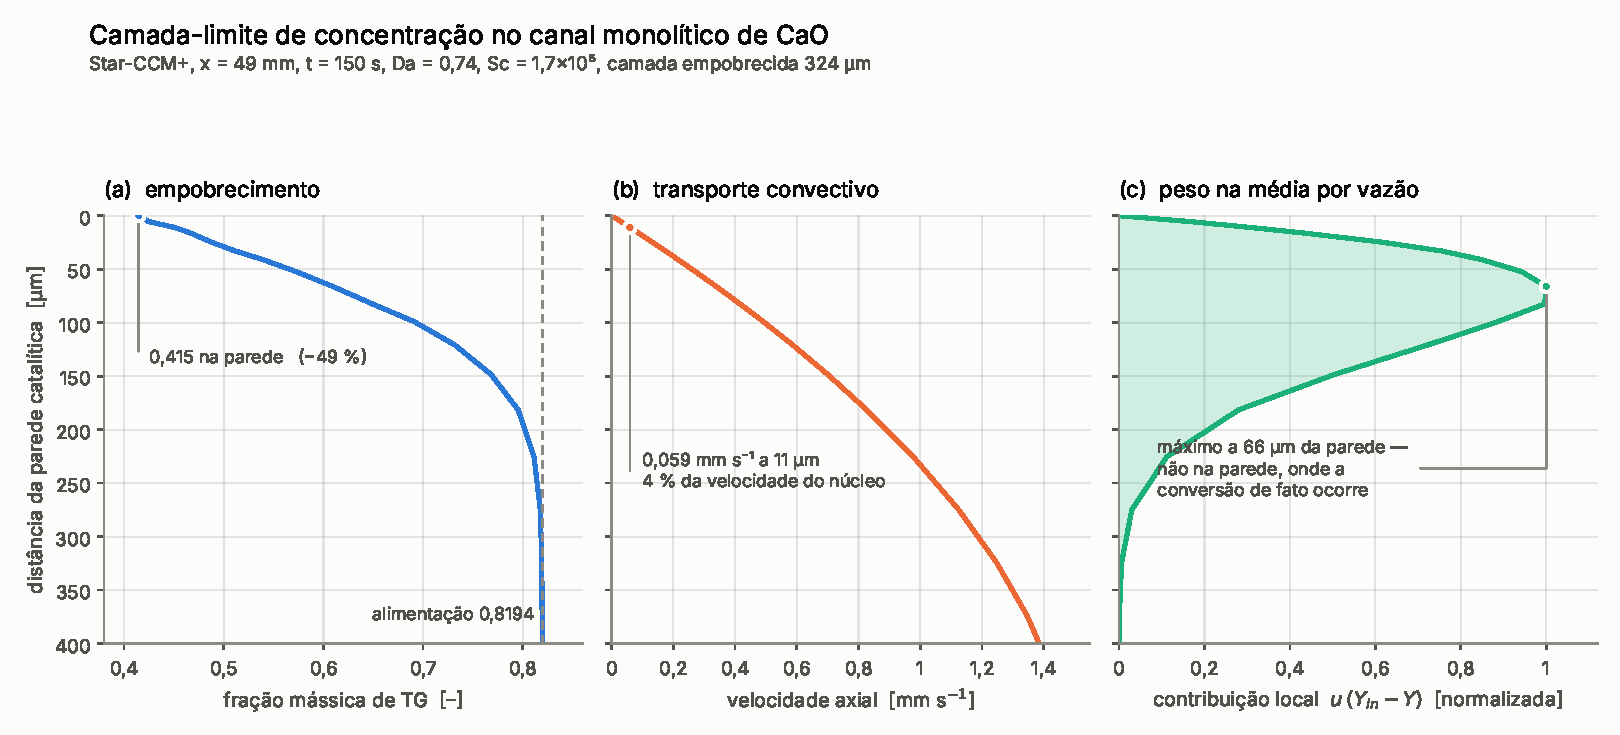
\includegraphics[width=\textwidth]{fig4_camada_limite_x49mm.pdf}
\caption{Camada-limite de concentração no canal monolítico de CaO, a
\SI{49}{\milli\meter} da entrada. (a)~fração mássica de triglicerídeo;
(b)~perfil de velocidade axial; (c)~contribuição local à média ponderada por
vazão}
\label{fig:camadalimite}
\end{figure}

A camada empobrecida tem espessura de \SI{324}{\micro\meter}, contra os
\SI{179}{\micro\meter} previstos pela solução de Lévêque,
Equação~\eqref{eq:leveque}, para regime permanente. A diferença tem origem
cinemática. Em \SI{150}{\second} de simulação, o regime permanente ainda não se
estabeleceu junto à parede, onde a velocidade local é muito pequena: o tempo de
trânsito do fluido situado a \SI{20}{\micro\meter} da superfície é de
\SI{458}{\second}, e a \SI{5}{\micro\meter}, de \SI{1833}{\second}. O tempo
característico do problema não é, portanto, o tempo de residência médio, igual a
$L/\bar{u} = \SI{50}{\second}$, mas o tempo de trânsito na região lenta, uma a
duas ordens de grandeza maior. Essa observação é relevante para o planejamento
de simulações futuras e para a interpretação de ensaios experimentais em
regime transiente.

O painel (c) da Figura~\ref{fig:camadalimite} merece comentário à parte. A
contribuição local à média ponderada por vazão, dada pelo produto
$u\,(Y_{\text{ent}} - Y)$, apresenta máximo a \SI{66}{\micro\meter} da parede, e
não sobre ela. A razão é simples e tem consequências que serão exploradas na
Seção~\ref{sec:reports}: o fluido mais empobrecido é justamente o mais lento, de
modo que a região onde a conversão de fato ocorre é a que menos pesa em qualquer
média ponderada pela vazão.

\section{Conversão por passe e limitação geométrica}

A conversão de triglicerídeo foi obtida diretamente da integral do fluxo de
parede,

\begin{equation}
X_{TG} = \frac{\left| \oint_{A_p} J_{TG}\, \mathrm{d}A \right|}{\dot{m}\, Y_{TG,\text{ent}}}
= \SI{1.40}{\percent}
\label{eq:conversao}
\end{equation}

\noindent
valor próximo de \SI{1.5}{\percent}, estimado analiticamente antes da simulação
pela combinação da solução de Lévêque com a cinética de parede.

O valor baixo não constitui deficiência do catalisador, e sim consequência
direta da relação entre o comprimento do canal e o comprimento de entrada
mássica. Com os parâmetros da Tabela~\ref{tab:propriedades},

\begin{align}
Re &= \frac{\rho\,\bar{u}\,D_h}{\mu} = 0{,}182 \nonumber\\
Sc &= \frac{\mu}{\rho\,D} = \num{1.73e5} \nonumber\\
Pe &= Re \cdot Sc = \num{3.1e4} \nonumber
\end{align}

\noindent
de modo que a Equação~\eqref{eq:entrada} fornece

\begin{equation}
L_e \approx 0{,}05 \times \SI{2.2e-3}{\meter} \times \num{3.1e4} = \SI{3.46}{\meter}
\end{equation}

\noindent
contra os \SI{50}{\milli\meter} do canal simulado, razão de \num{69}. A
camada-limite de concentração jamais chega a preencher a seção, e o núcleo do
escoamento deixa o canal praticamente na composição de alimentação.

Trata-se, a rigor, do resultado de projeto mais consequente obtido até aqui. O
número de Schmidt elevado, característico de óleos vegetais, implica que um
canal curto opera permanentemente na região de entrada mássica. Elevar a
conversão por passe exige atuar sobre $Pe$ ou sobre $L$, seja por meio de canais
mais longos, de velocidade superficial menor ou de reciclo. Aumentar
isoladamente a carga de catalisador tem retorno decrescente, uma vez que, já em
$Da = \num{0.76}$, o transporte externo responde por \SI{43}{\percent} da queda
de concentração disponível.

\section{Considerações metodológicas sobre a leitura de grandezas de fronteira}
\label{sec:reports}

O fechamento do balanço de massa descrito na Equação~\eqref{eq:balanco} exigiu
esforço desproporcional à sua aparente simplicidade, e as dificuldades
encontradas têm interesse que ultrapassa o presente trabalho. Registram-se aqui
por constituírem modos de falha que não se manifestam em nenhum dos indicadores
usuais de convergência.

Ao longo das simulações, três relatórios distintos de fração mássica de espécie,
todos avaliados em face de fronteira ou em objeto derivado, forneceram valores
incorretos, retornando aproximadamente a composição de alimentação. Em
contrapartida, as grandezas avaliadas sobre células permaneceram corretas e
mutuamente consistentes. A Tabela~\ref{tab:reports} sintetiza o comportamento
observado.

\begin{table}[htb]
\centering
\caption{Confiabilidade das grandezas de fração mássica avaliadas}
\label{tab:reports}
\begin{tabular}{l l l}
\toprule
Grandeza & Base de avaliação & Comportamento \\
\midrule
Média volumétrica de $Y_i$              & célula (região)        & correta \\
Integral de superfície de $J_i$         & função de campo        & correta \\
Média de superfície de $Y_i$ na parede  & face de fronteira      & retornou $Y_{\text{ent}}$ \\
Média ponderada por vazão na saída      & face de fronteira      & erro de fator \num{19} \\
Sonda de linha de $Y_i$                 & objeto derivado        & retornou $Y_{\text{ent}}$ \\
\bottomrule
\end{tabular}
\end{table}

O caso da média ponderada por vazão na saída possui, além da falha numérica, uma
fragilidade de natureza física já antecipada na Seção~\ref{sec:camadalimite}: o
fluido mais empobrecido é o mais lento, de modo que a região portadora da
informação de conversão quase não pesa na média, e o resultado fica à mercê de
qualquer contaminação pela composição especificada na fronteira.

Uma distinção útil emergiu da última corrida. O monitor de média de superfície
sobre a parede, isto é, a série temporal registrada a cada passo, permaneceu
cravado no valor da alimentação do primeiro ao último instante, ao passo que o
relatório instantâneo da mesma grandeza, consultado ao fim da corrida, forneceu
o valor correto de \num{0.481093}, confirmado pela integral do fluxo em seis
algarismos. Monitor e relatório podem, portanto, divergir, e a verificação
cruzada da Equação~\eqref{eq:cruzada} deve ser aplicada a ambos.

O caso da média de superfície sobre a parede é inequívoco. Ao retomar-se a
marcha a partir de um arquivo salvo, o relatório passou a retornar o valor exato
da composição de alimentação, \num{0.819400}, permanecendo congelado por três
mil passos de tempo, ao passo que a integral do fluxo sobre a mesma parede
seguia correta e fornecia, pela cadeia de funções de campo,
$Y_{TG}|_{\text{parede}} = \num{0.4521}$. Uma sonda de linha criada após a
retomada apresentou o mesmo defeito.

A prática que se consolidou ao longo do trabalho, e que se recomenda a quem
venha a montar modelos semelhantes, é a seguinte. Para fração mássica de
espécie, empregam-se exclusivamente grandezas avaliadas sobre células, a saber,
médias e integrais volumétricas sobre a região, e integrais de superfície de
funções de campo construídas sobre o próprio campo. A verificação cruzada que
detecta os três casos é barata e deve ser executada de rotina:

\begin{equation}
\text{média volumétrica de } Y_i \;\;\stackrel{!}{=}\;\; \frac{M_i}{\rho\, V}
\label{eq:cruzada}
\end{equation}

\noindent
com concordância esperada de cinco a seis algarismos significativos. Não havendo
concordância, o erro está no relatório, e não no modelo.

\chapter{Resultados Esperados e Cronograma de Atividades}
\label{cap:cronograma}

\section{Resultados esperados}

O modelo descrito no Capítulo~\ref{cap:modelagem} encontra-se verificado e
operacional, e os resultados do Capítulo~\ref{cap:resultados} estabelecem o
regime de operação do sistema. As etapas restantes do trabalho destinam-se a
substituir as estimativas ainda empregadas por dados medidos, a explorar o
espaço de parâmetros de projeto e a confrontar o modelo com a resposta
experimental do reator.

\subsection{Substituição dos parâmetros estimados}

Três grandezas do modelo são hoje estimativas, e cada uma delas será substituída
por medida experimental assim que disponível.

A massa específica e a espessura do \textit{washcoat} entram no modelo apenas
pelo produto $\rho_{wc}\,\delta_{wc}$, ao qual a taxa de reação é linearmente
proporcional, conforme as Equações~\eqref{eq:rw} e~\eqref{eq:w}. Sua
caracterização é, por essa razão, a medida de maior retorno imediato para a
acurácia do modelo, e espera-se que a incerteza associada ao número de Damköhler
caia proporcionalmente.

As dimensões do canal, hoje tomadas de valores típicos de monólitos comerciais,
serão medidas nas peças efetivamente disponíveis no laboratório. A altura e o
comprimento do canal deixaram de ser parâmetros secundários a partir do momento
em que se verificou que o comprimento de entrada mássica supera o comprimento
físico em quase duas ordens de grandeza; espera-se que a razão $L_e/L$ se
mantenha elevada, mas seu valor exato determina a magnitude da limitação
geométrica discutida no Capítulo~\ref{cap:resultados}.

As propriedades físicas do meio reacional, por fim, serão obtidas para a carga
efetivamente empregada, em lugar dos valores de literatura hoje adotados.

\subsection{A geometria do monólito disponível}
\label{sec:geomreal}

Durante a redação deste texto, as dimensões das peças de suporte efetivamente
disponíveis no laboratório foram medidas e repassadas pela orientação. Diferem
de forma apreciável da geometria de referência adotada nas simulações
apresentadas, e merecem registro por condicionarem as etapas seguintes.

\begin{table}[htb]
\centering
\caption{Geometria simulada e geometria das peças disponíveis}
\label{tab:geomreal}
\begin{tabular}{l c c}
\toprule
 & Simulado & Peça disponível \\
\midrule
Seção do canal          & plano          & quadrado \\
Abertura                & \SI{1.1}{\milli\meter} & \SI{0.55}{\milli\meter} \\
Comprimento             & \SI{50}{\milli\meter}  & \SI{29.15}{\milli\meter} \\
Paredes catalíticas     & \num{1}        & \num{4} \\
Espessura de parede     & ---            & \SI{0.10}{\milli\meter} \\
Densidade de células    & \num{400} cpsi & \num{1527} cpsi \\
\bottomrule
\end{tabular}
\end{table}

A geometria simulada derivou de \textcite{Asli2011}, como exposto no
Capítulo~\ref{cap:revisao}. A peça disponível tem metade da abertura, seção
quadrada com as quatro paredes recobertas e densidade de células quase quatro
vezes maior.

Estimativas preliminares, obtidas por extrapolação do modelo verificado através
da solução de Lévêque e do balanço de área, indicam que o canal menor engrossa
menos a camada-limite e eleva o coeficiente de transferência de massa em cerca
de \SI{50}{\percent}. O número de Damköhler cairia de \num{0.76} para
aproximadamente \num{0.51}, permanecendo em regime misto, e a conversão por
passe de uma peça subiria de \SI{1.4}{\percent} para algo próximo de
\SI{7.7}{\percent}, sobretudo pelo aumento de oito vezes na razão entre área de
parede e volume. O comprimento de entrada mássica cairia para
\SI{216}{\milli\meter}, ainda sete vezes o comprimento da peça.

Dessa última razão decorre uma consequência de projeto. Operando na região de
entrada, o coeficiente de transferência de massa decai com $x^{-1/3}$, de modo
que empilhar peças curtas com desalinhamento entre elas, de forma que a
camada-limite se reinicie a cada peça, eleva o coeficiente médio por um fator
$N^{1/3}$ em relação a um canal contínuo de mesmo comprimento total. Para trinta
peças, fator próximo de três. A verificação dessa estimativa por simulação da
geometria real consta das atividades previstas.

\subsection{Varredura paramétrica}

Com o modelo calibrado, pretende-se realizar varreduras em três direções.

A espessura do \textit{washcoat} será variada de modo a localizar o joelho da
curva de saturação descrita pela Equação~\eqref{eq:saturacao}, que define a
faixa de deposição economicamente razoável. A análise preliminar da
Seção~\ref{sec:thiele} indica \SIrange{10}{15}{\micro\meter}, e espera-se que
a varredura confirme essa faixa com o valor medido de $D_p$ e forneça um número
que possa orientar o procedimento de impregnação.

A temperatura será varrida na faixa compatível com a operação em metanol à
pressão atmosférica. Essa varredura exige a substituição da constante cinética
por uma expressão de Arrhenius, o que depende da energia de ativação a ser
obtida experimentalmente. Espera-se observar o deslocamento do número de
Damköhler com a temperatura, dado que a cinética é mais sensível a $T$ do que a
difusividade, e portanto a transição gradual do regime misto em direção ao
controle por transporte à medida que a temperatura se eleva.

A geometria do canal será reconstruída segundo as dimensões da
Tabela~\ref{tab:geomreal}, o que exige abandonar a formulação pseudo-bidimensional
em favor de um quarto de duto quadrado, aproveitando os dois planos de simetria.
A física, as funções de campo e o protocolo de verificação do
Capítulo~\ref{cap:modelagem} transferem-se sem alteração; mudam a geometria e a
malha. Em seguida, comprimento e abertura serão variados em torno desses valores,
e o efeito do desalinhamento entre peças sucessivas será avaliado.

\subsection{Calibração e confronto com dados experimentais}

Os ensaios em condução no laboratório fornecerão conversões medidas em condições
controladas de temperatura, razão molar e vazão. O confronto entre essas
conversões e as previstas pelo modelo permitirá ajustar os parâmetros ainda
incertos, em particular a difusividade efetiva do triglicerídeo no meio e no
poro, e estabelecer a faixa de validade do modelo.

Espera-se que o modelo reproduza a tendência experimental de conversão com a
vazão, dado que essa dependência é governada pelo transporte externo, que o
modelo resolve explicitamente. Discrepâncias sistemáticas, caso ocorram, serão
examinadas à luz das hipóteses listadas na Seção~\ref{sec:difusividades},
notadamente a de difusividades iguais entre espécies, cuja substituição pela
formulação de Maxwell-Stefan constitui a alternativa prevista.

\subsection{Decisão quanto à rota alcoólica}

Permanece em aberto a definição da rota a ser modelada em definitivo. A rota
metílica, à qual correspondem os parâmetros de \textcite{Melo2023} empregados
até aqui, opera a \SI{65}{\celsius} com razão molar de \num{4}:\num{1}. A rota
etílica, estudada por \textcite{Fonseca2026} a \SI{70}{\celsius} e razão de
\num{1}:\num{9}, apresenta vantagens de origem da matéria-prima no contexto
brasileiro, mas cinética mais lenta e separação mais difícil. A decisão será
tomada em conjunto com a orientação, e o modelo está estruturado de modo a
acomodar qualquer das duas sem alteração de sua formulação.

\section{Cronograma de atividades}

A Tabela~\ref{tab:cronograma} apresenta o cronograma proposto para a execução do
trabalho, considerando-se o período integral do mestrado.

\begin{table}[htb]
\centering
\caption{Cronograma proposto para as atividades do presente estudo}
\label{tab:cronograma}
\renewcommand{\arraystretch}{1.3}
\begin{tabular}{|l|c|c|c|c|c|c|}
\hline
\multirow{2}{*}{\textbf{Atividade}} & \multicolumn{6}{c|}{\textbf{Semestre / Ano}} \\
\cline{2-7}
 & \textbf{1º/25} & \textbf{2º/25} & \textbf{1º/26} & \textbf{2º/26} & \textbf{1º/27} & \textbf{2º/27} \\
\hline
Disciplinas obrigatórias        & \cellcolor{gray!55} & \cellcolor{gray!55} & \cellcolor{gray!55} & \cellcolor{gray!55} &  &  \\
\hline
Revisão bibliográfica           & \cellcolor{gray!55} & \cellcolor{gray!55} & \cellcolor{gray!55} & \cellcolor{gray!55} & \cellcolor{gray!55} &  \\
\hline
Desenvolvimento do modelo CFD   &  & \cellcolor{gray!55} & \cellcolor{gray!55} & \cellcolor{gray!55} &  &  \\
\hline
Verificação do modelo           &  &  & \cellcolor{gray!55} & \cellcolor{gray!55} &  &  \\
\hline
Exame de qualificação           &  &  &  & \cellcolor{gray!55} &  &  \\
\hline
Caracterização do catalisador   &  &  &  & \cellcolor{gray!55} & \cellcolor{gray!55} &  \\
\hline
Ensaios experimentais           &  &  &  & \cellcolor{gray!55} & \cellcolor{gray!55} &  \\
\hline
Calibração do modelo            &  &  &  &  & \cellcolor{gray!55} &  \\
\hline
Varredura paramétrica           &  &  &  &  & \cellcolor{gray!55} & \cellcolor{gray!55} \\
\hline
Análise dos resultados          &  &  &  &  & \cellcolor{gray!55} & \cellcolor{gray!55} \\
\hline
Redação e defesa da dissertação &  &  &  &  &  & \cellcolor{gray!55} \\
\hline
\end{tabular}
\end{table}

\pendente{conferir as datas de início do mestrado e de integralização dos
créditos, e ajustar o cronograma à previsão de defesa acordada com a orientação}


% ============================== REFERÊNCIAS ==================================
\cleardoublepage
\markboth{Referências Bibliográficas}{}
\addcontentsline{toc}{chapter}{Referências Bibliográficas}
\printbibliography[title=Referências Bibliográficas]

\end{document}
